\chapter{Inference on Czech News}\label{inference}
Finally, the classifier built in the previous section is used to classify media bias in the Czech news corpus. The results across different domains, sections, and granularities are presented.



\section{Data}
For this purpose, the \textbf{SumeCzech}\footnote{\url{https://ufal.mff.cuni.cz/sumeczech}} dataset has been used \cite{straka2018sumeczech}. It is originally a dataset meant for training summarization models; however, it consists of complete news articles in JSON format and therefore is suitable.

The dataset includes five Czech news domains: novinky.cz, idnes.cz, ceskenoviny.cz, denik.cz, lidovky.cz. 

A list of the fields available in the dataset can be seen in the following:
\begin{itemize}
    \item \verb|text :| body of the article
    \item \verb|headline :| headline of the article
    \item \verb|abstract :|  abstract of the article
    \item \verb|subdomain :| domains with some additional information about the topics, e.g. lidovky.cz has sport.lidovky.cz for sport news.
    \item \verb|section :| a topic of the article
    \item \verb|published :| date of publication
    \item \verb|length :| number of characters in the text
\end{itemize}



\section{Pre-processing}
The SumeCzech contains around one million articles. For the experiments, I only used the validation and test split, which comprises approximately 90k articles. Furthermore, only data from the ceskenoviny.cz domain were oversampled from the large train set to match the size of other domains.

All subdomains were stripped such that only a domain remained. The prefix of the domain was additionally imputed as a section. See an example in the following:
\begin{verbatim}
    subdomain:= novinky.cz <- sport.novinky.cz 
    section:= sport <- sport.novinky.cz
\end{verbatim}

Also, I decided to exclude all blogs. Therefore, all the data that contained the 'blog' substring in its subdomain were removed.

To balance the domains, I sampled 4000 articles from each domain, resulting in a final dataset consisting of 20000 articles.


\section{Methodology}
For each article in the dataset, the following procedure was executed:
\begin{enumerate}
    \item Text and abstract are splitted into sentences using \verb|sent_tokenize| nltk function\footnote{\url{https://www.nltk.org/}}.
    \item Each sentence from the text, abstract and a headline is classified with binary label 0,1 using the media bias classifier (\ref{classifier}).
    \item Each sentence from the text is assigned with 'reported\_speech' indicator if matched the regular expression for quoting extraction. 
    \item The precentage of biased sentences is calculated for text and abstract.
    \item The percentage of reported speech among the sentences is calculated for the text.
\end{enumerate}

This procedure results in the introduction of four new fields:
\begin{itemize}
    \item \verb|text_bias :| percentage of biased sentences in the text
    \item \verb|abstract_bias :| percentage of biased sentences in the abstract
    \item \verb|headline_bias :| bias label of the headline
    \item \verb|quoting_ratio :| percentage of reported speech in the text     
\end{itemize}



These fields are further used to study the nature of the media bias in the corpus.
For data processing and statistics, third-party libraries were used, in particular, \textbf{numpy}\footnote{\url{https://numpy.org/}}, \textbf{pandas}\footnote{\url{https://pandas.pydata.org/}}, \textbf{scipy}\footnote{\url{https://scipy.org/}} for data processing and \textbf{seaborn}\footnote{\url{https://seaborn.pydata.org/}} for visualizations.


\section{Results}
In this section I present statistics of media bias across domains and topics and, additionally, its progression over time for the denik.cz domain.

%%%%% CORR %%%%%
\subsection{Correlations}
Firstly, a simple correlation heatmap is shown in figure \ref{fig:corr}. Bias of the abstract and the headline has a relatively high correlation with the \verb|text_bias|. Both the abstract and the headline are a sort of an aggregate of the text; therefore, these results are justified.

Furthermore, there is some evidence that longer articles tend to be more biased, but the coefficient of correlation is relatively low.

Seemingly, there is no relationship between the \verb|quoting_ratio| (frequency of reported speech)
and the bias of the article.

\begin{figure}

  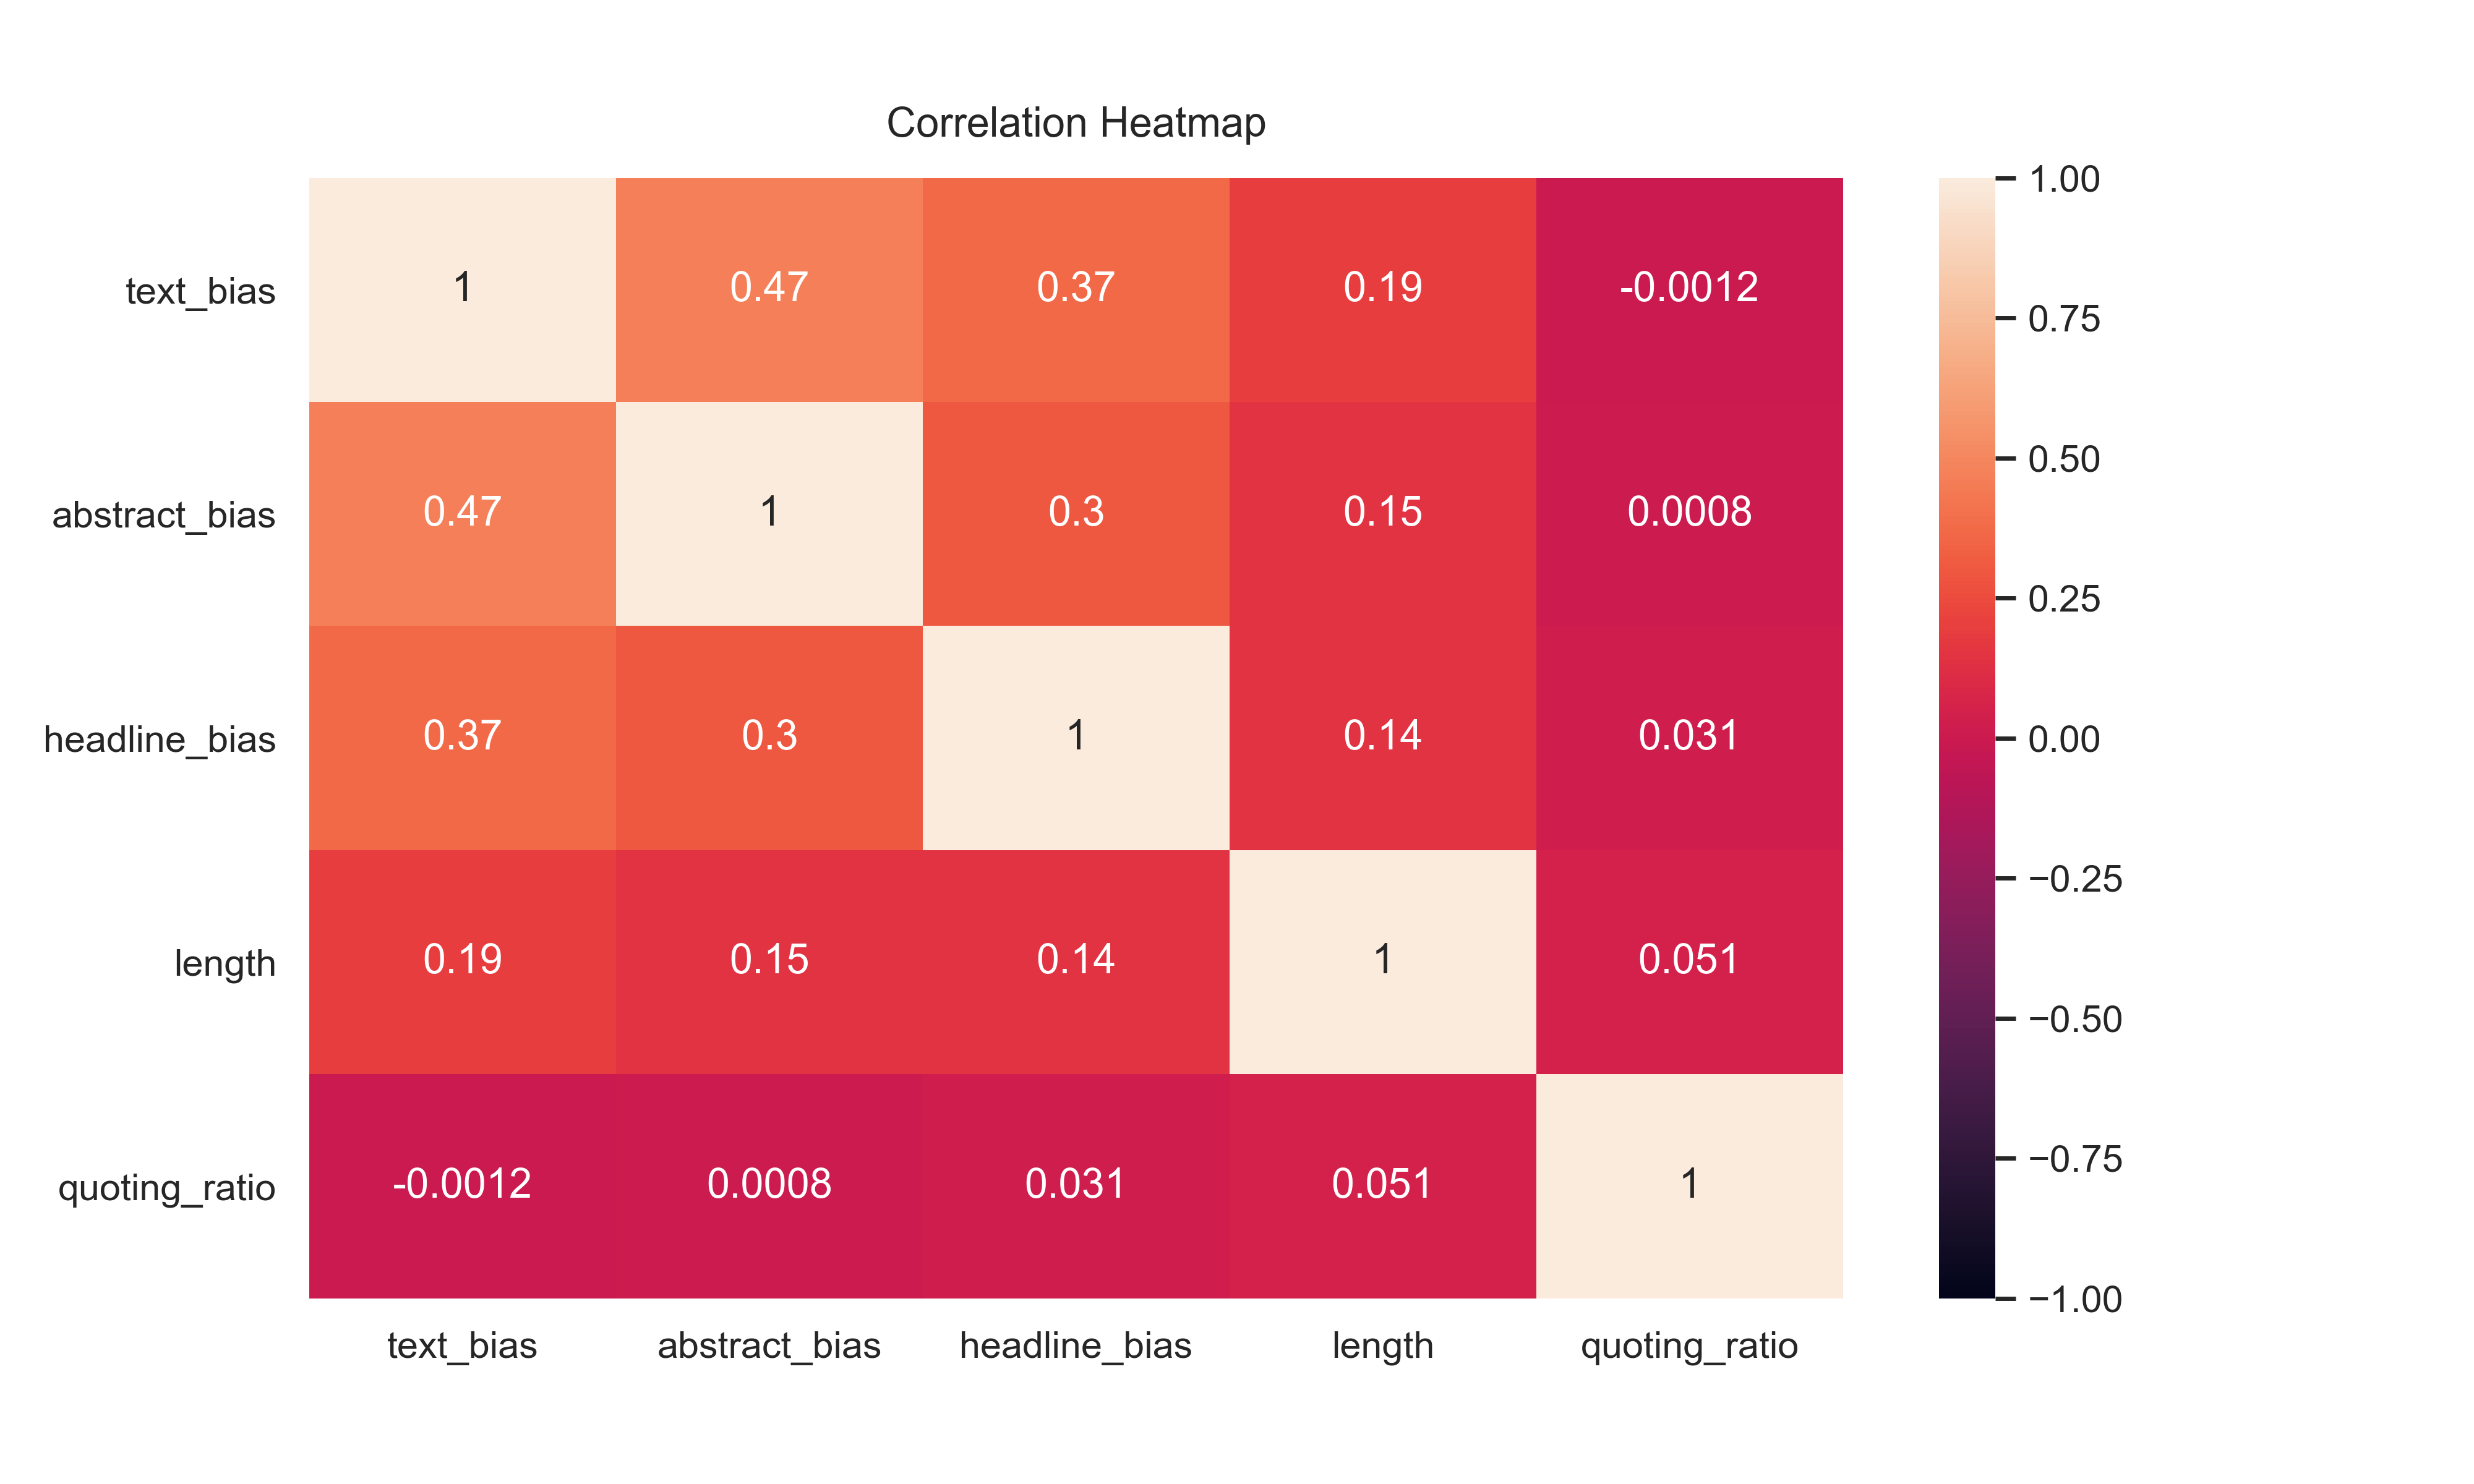
\includegraphics[scale=0.5]{my_modules/multimedia/inference/corr.png}
  \caption{Correlation of dataset fields.}
  \label{fig:corr}

\end{figure}


\subsection{Bias distribution}
Histogram of the \verb|text_bias| values can be seen in figure \ref{fig:dists}. In the first plot, we see that more than 20\% of the classified articles had no biased sentences at all. To have a more detailed look at the distribution, I omitted the unbiased articles in the second histogram. Apparently, most of the biased articles have between 5-10\% of biased sentences.


\begin{figure}

  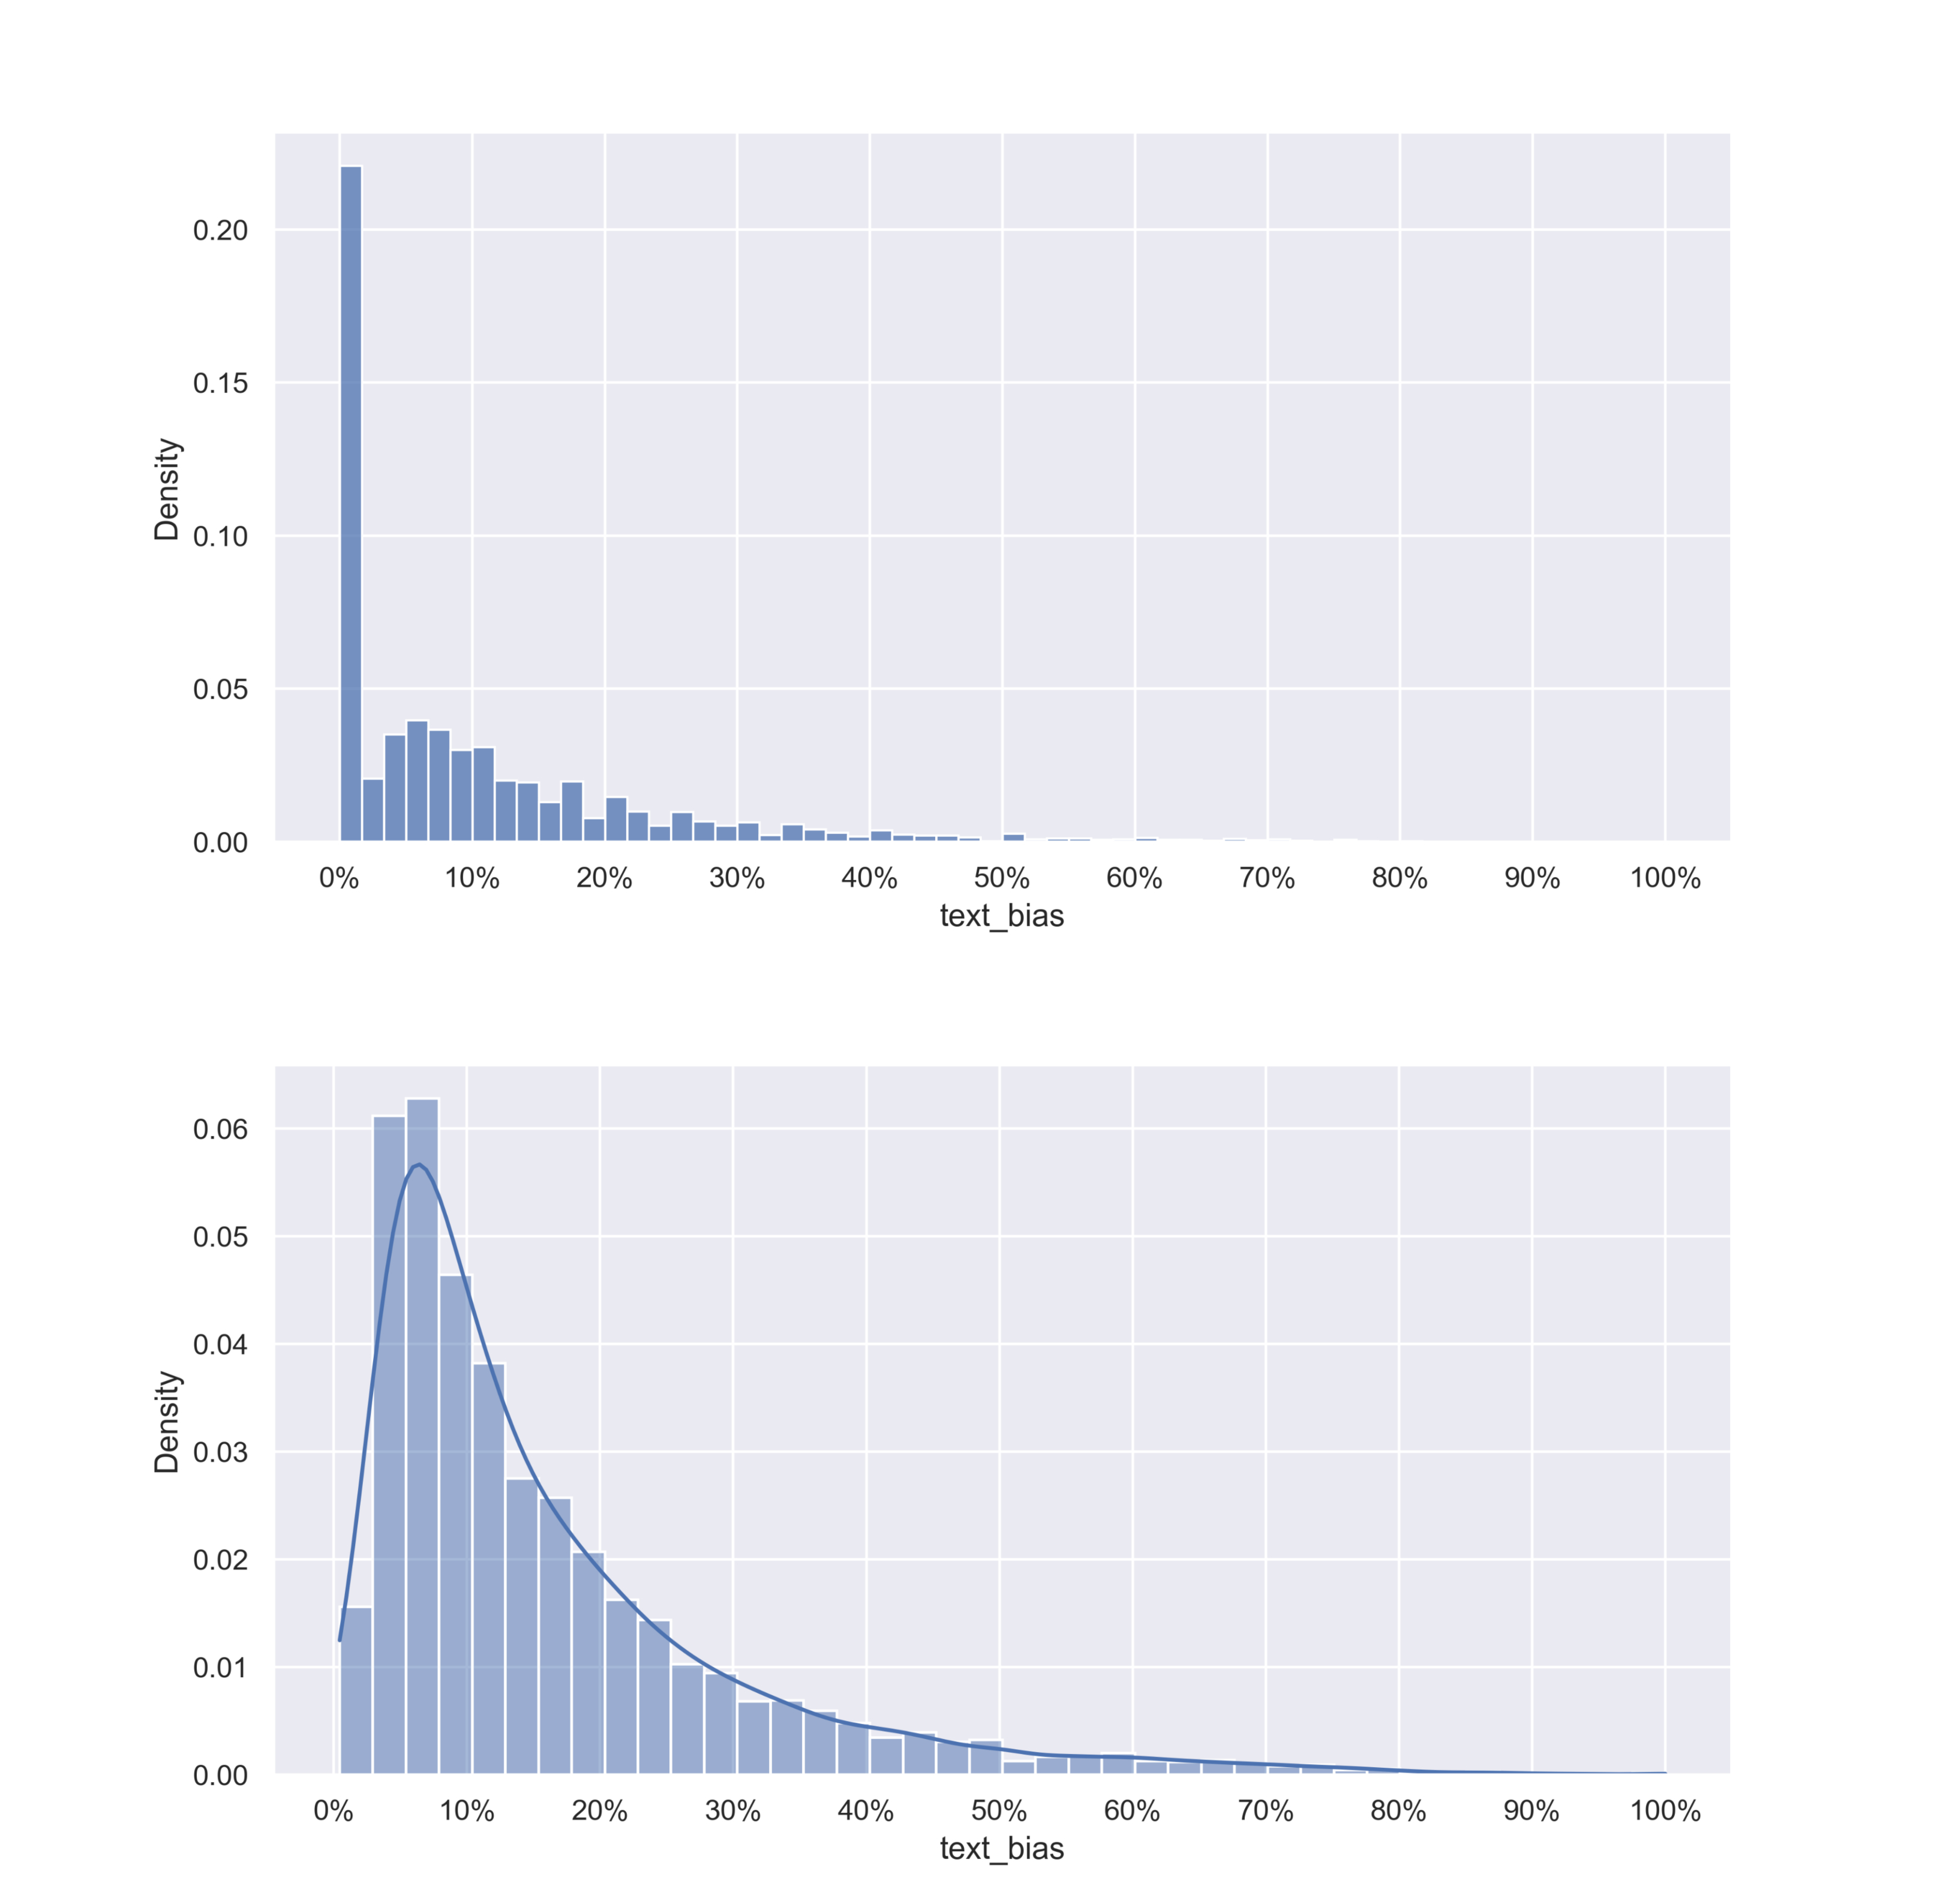
\includegraphics[scale=0.5]{my_modules/multimedia/inference/dists.jpg}
  \caption{Distribution of text bias values over the dataset. Second plot is without the articles with 0 text bias.}
  \label{fig:dists}

\end{figure}


\newpage
%%%%%%%%%%%%%%%%%%%%%%%%%% DOMAINS %%%%%%%%%%%%%%%%%%%%%%%%%%%%%%%%%%%%%%%
\subsection{Bias between domains}
To study the bias distribution between domains, the data was grouped by domains and their \verb|text_bias| and \verb|headline_bias| within the domain were averaged. The bar plot of the results can be seen in figure \ref{fig:domains}. \textbf{ceskenoviny.cz} exhibit significantly lower average \verb|text_bias| as well as the ratio of biased headlines (average \verb|headline_bias|).

Furthermore, the difference between the bias distribution of the least biased and the most biased domain is presented in the figure \ref{fig:dists_ctk_idnes}. An x-axis is log-scaled for better visualization.
\newpage


\begin{figure}

  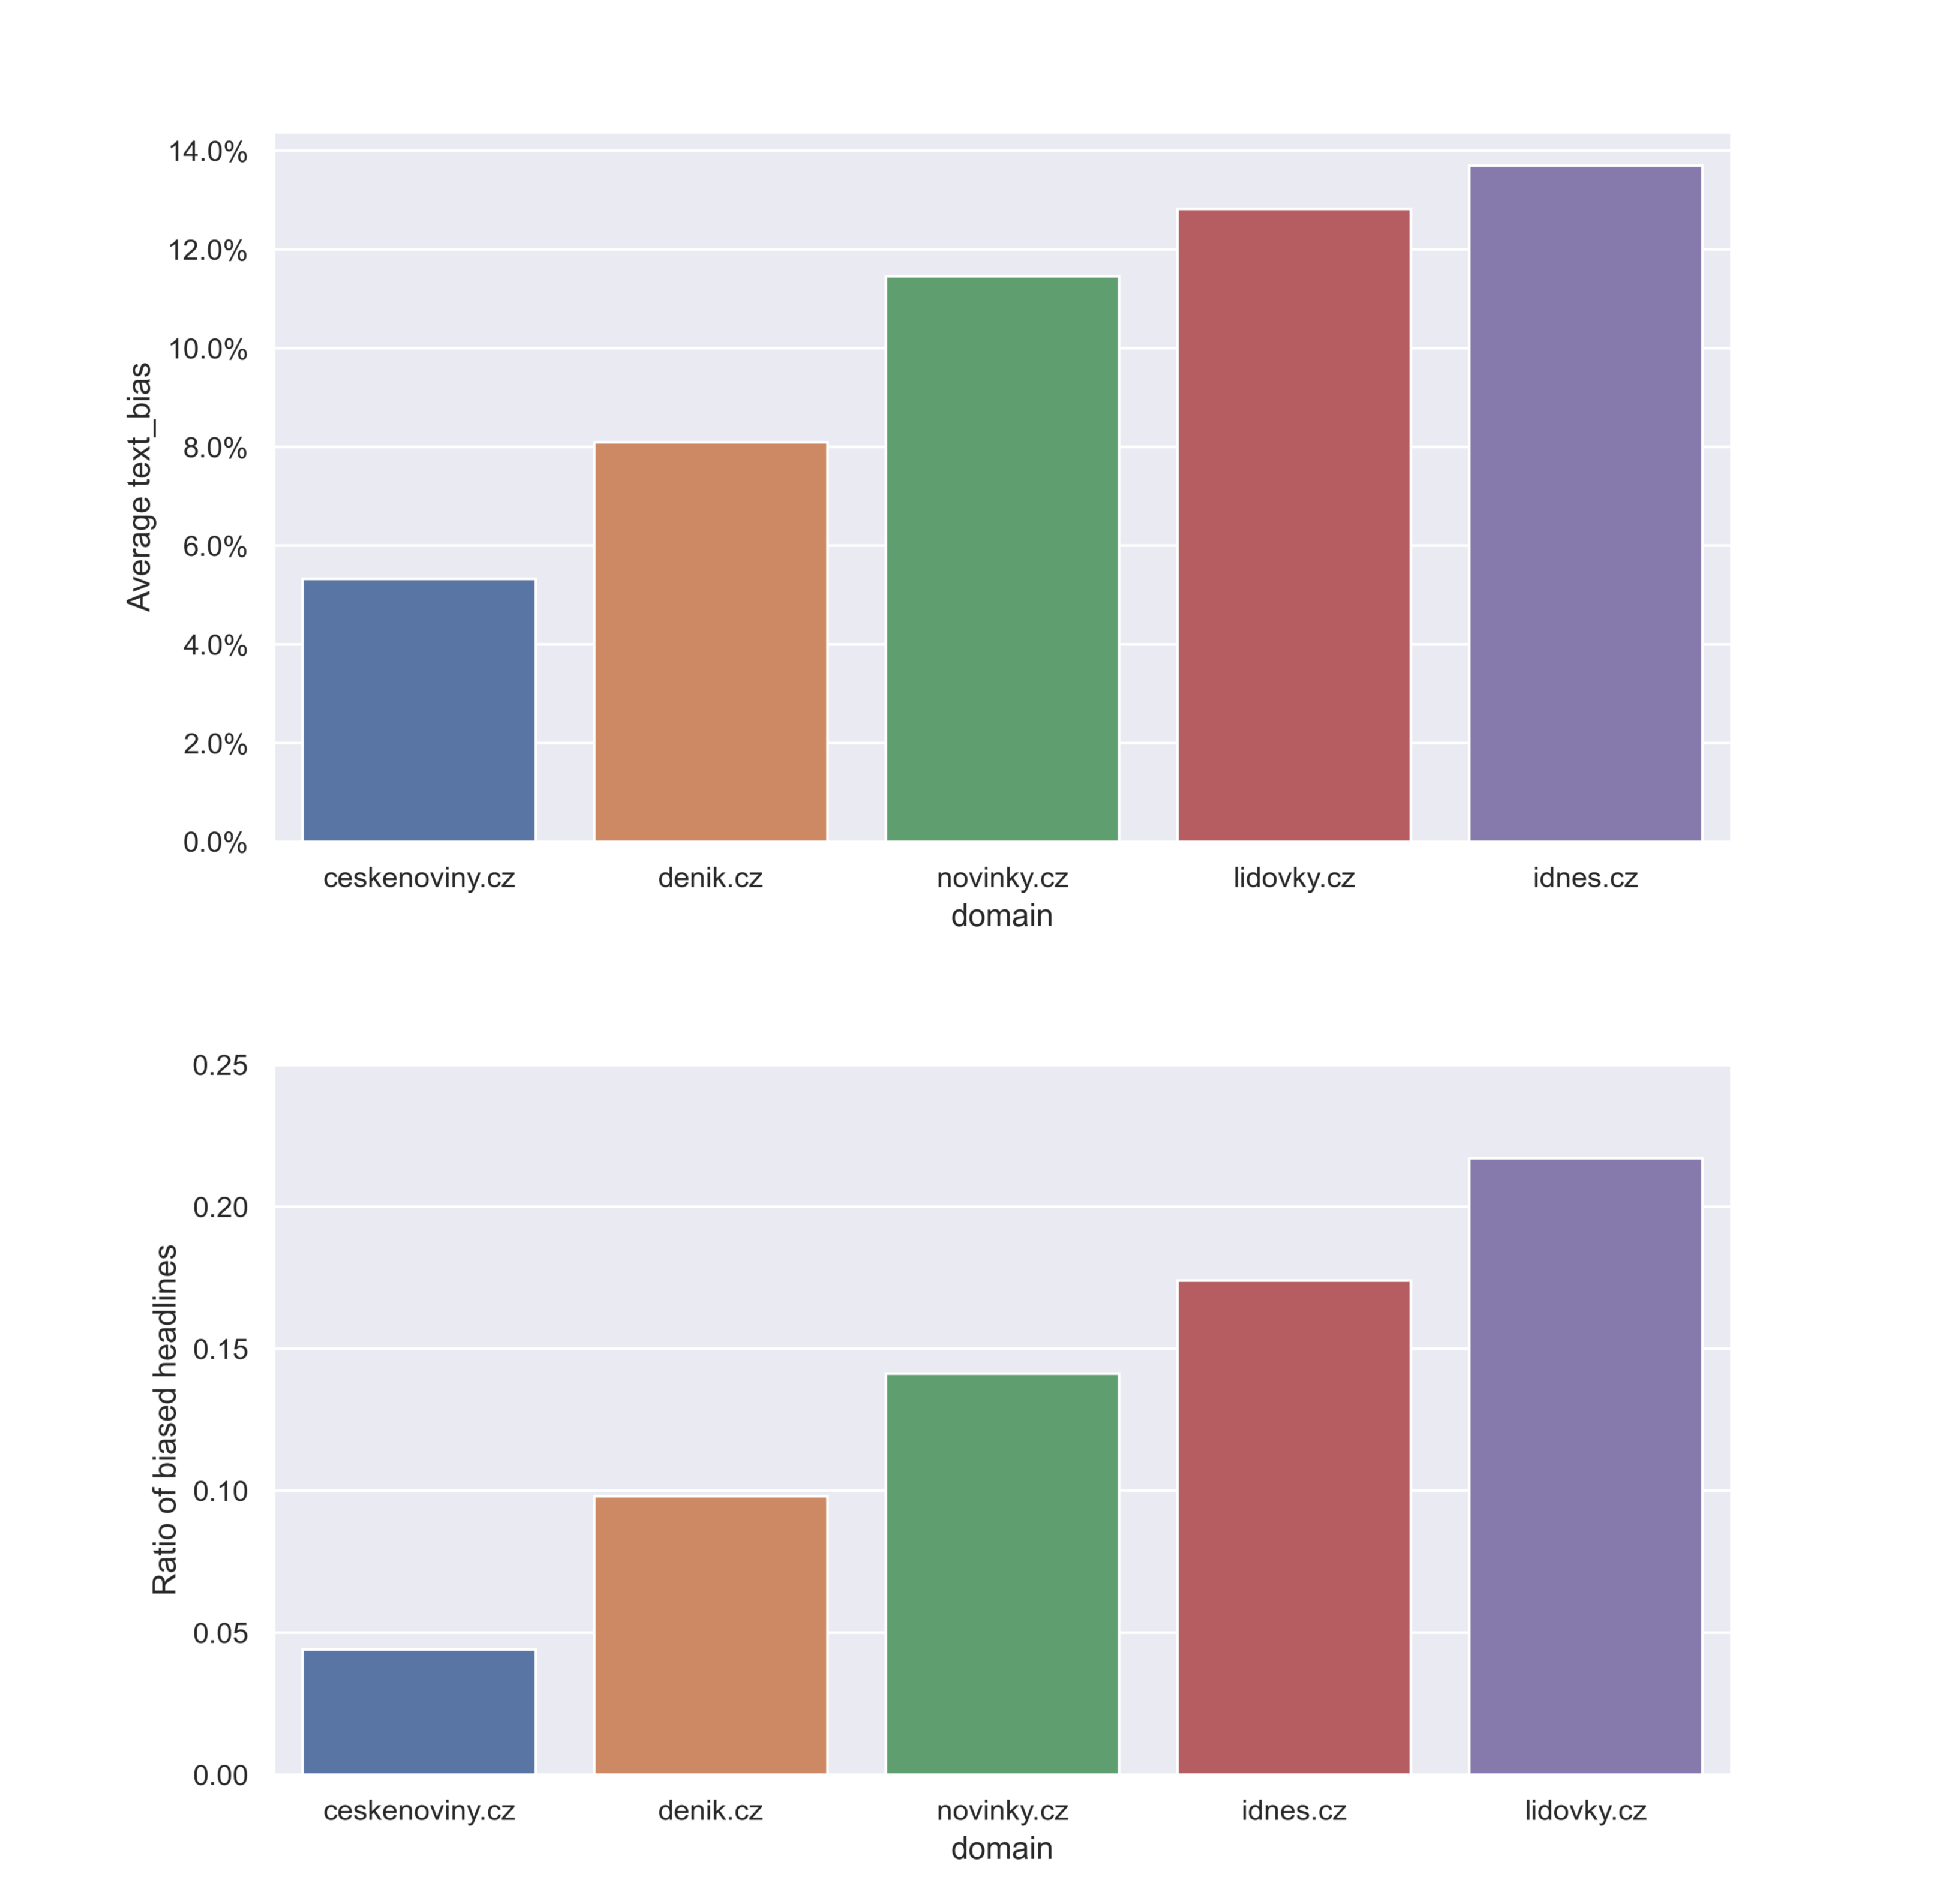
\includegraphics[scale=0.5]{my_modules/multimedia/inference/domains.jpg}
  \caption{Comparison of average text bias and headline bias across the domains.}
  \label{fig:domains}

\end{figure}

\begin{figure}
  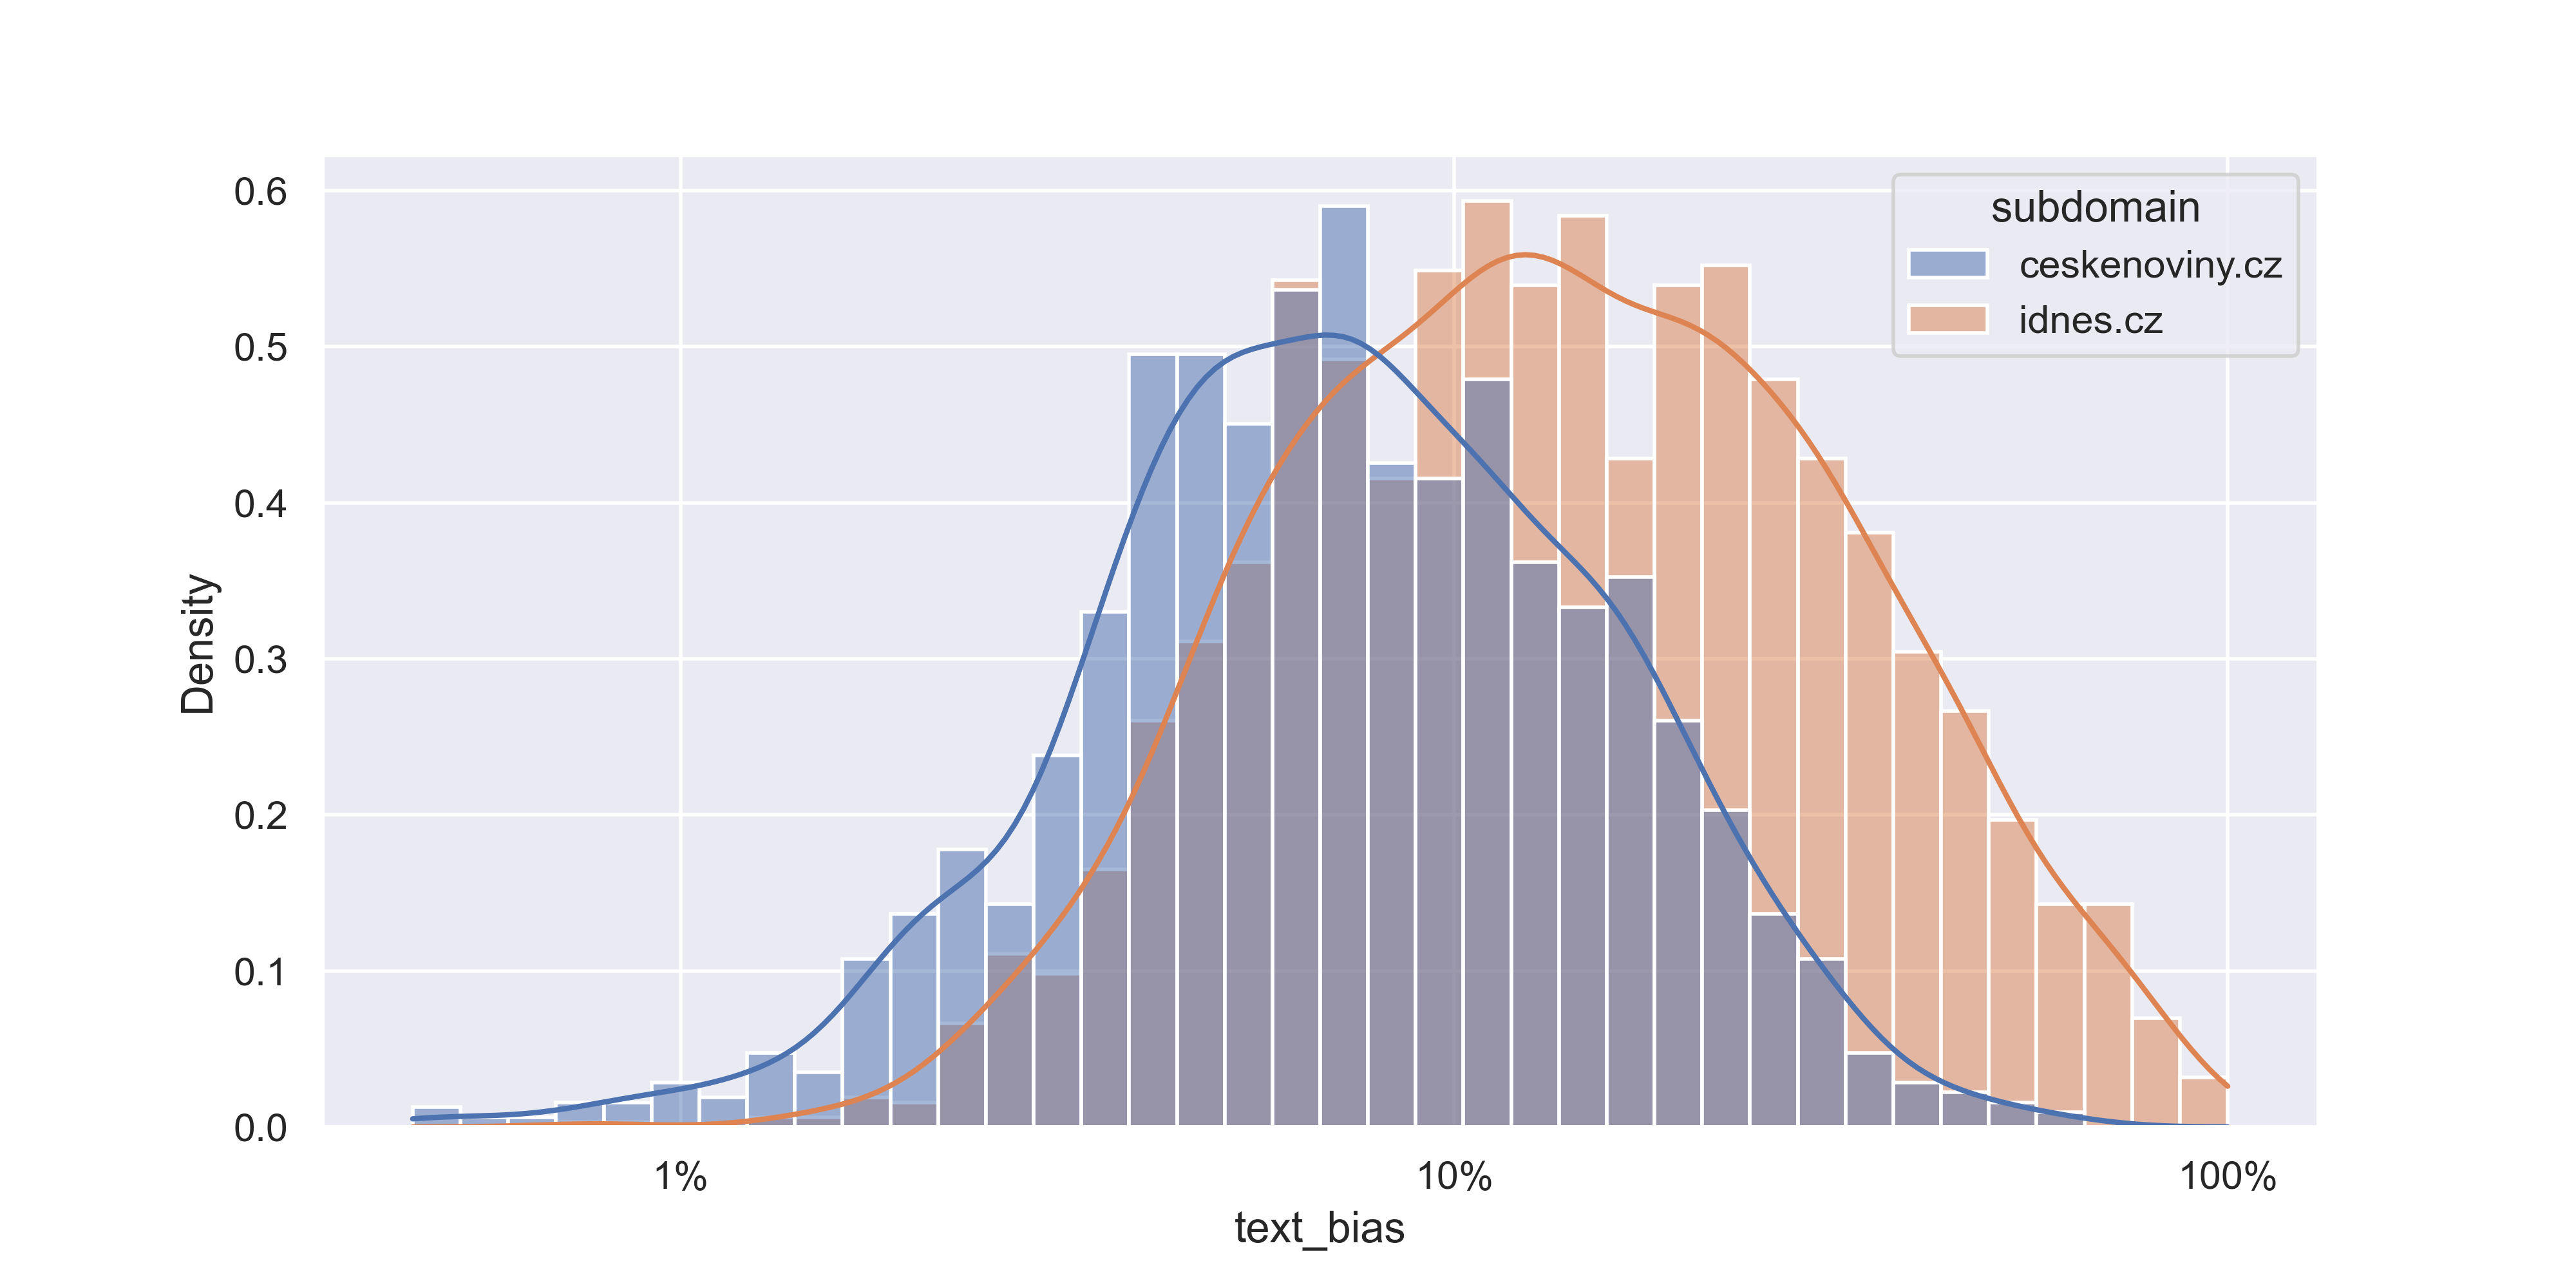
\includegraphics[scale=0.5]{my_modules/multimedia/inference/dists_ctk_idnes.png}
  \caption{Distributions of bias between two domains.}
  \label{fig:dists_ctk_idnes}
\end{figure}








\newpage
\subsection{Bias between sections}\label{commentary_bias}
In this experiment, data were grouped by sections (topics of the article) and their \verb|text_bias| was averaged. I made an arbitrary choice to exclude sections that had less than 50 data points within the dataset, because such sections were way too specific.

The ten least biased and most biased sections\footnote{\textit{rungo} is a lifestyle section, \textit{xman} is a male oriented section and \textit{revue} is sort of a yellow press.} can be seen in figure \ref{fig:sections}. The values are in percents.


Sections that exhibit low average \verb|text_bias|, for example \textit{career}, \textit{economics}, \textit{business} are all of a rather factual, emotionless nature.
On the other hand, sections with high average bias, such as \textit{art}, \textit{music}, and \textit{culture}, are more of a subjective, personal nature.

Interestingly, the \textit{commentary} section, exhibits by far the highest average \verb|text_bias| (51.97\%). This was an expected result, as the essence of the \textit{commentary} format is to present an opinion, often subjective.

%\begin{figure}
%
%  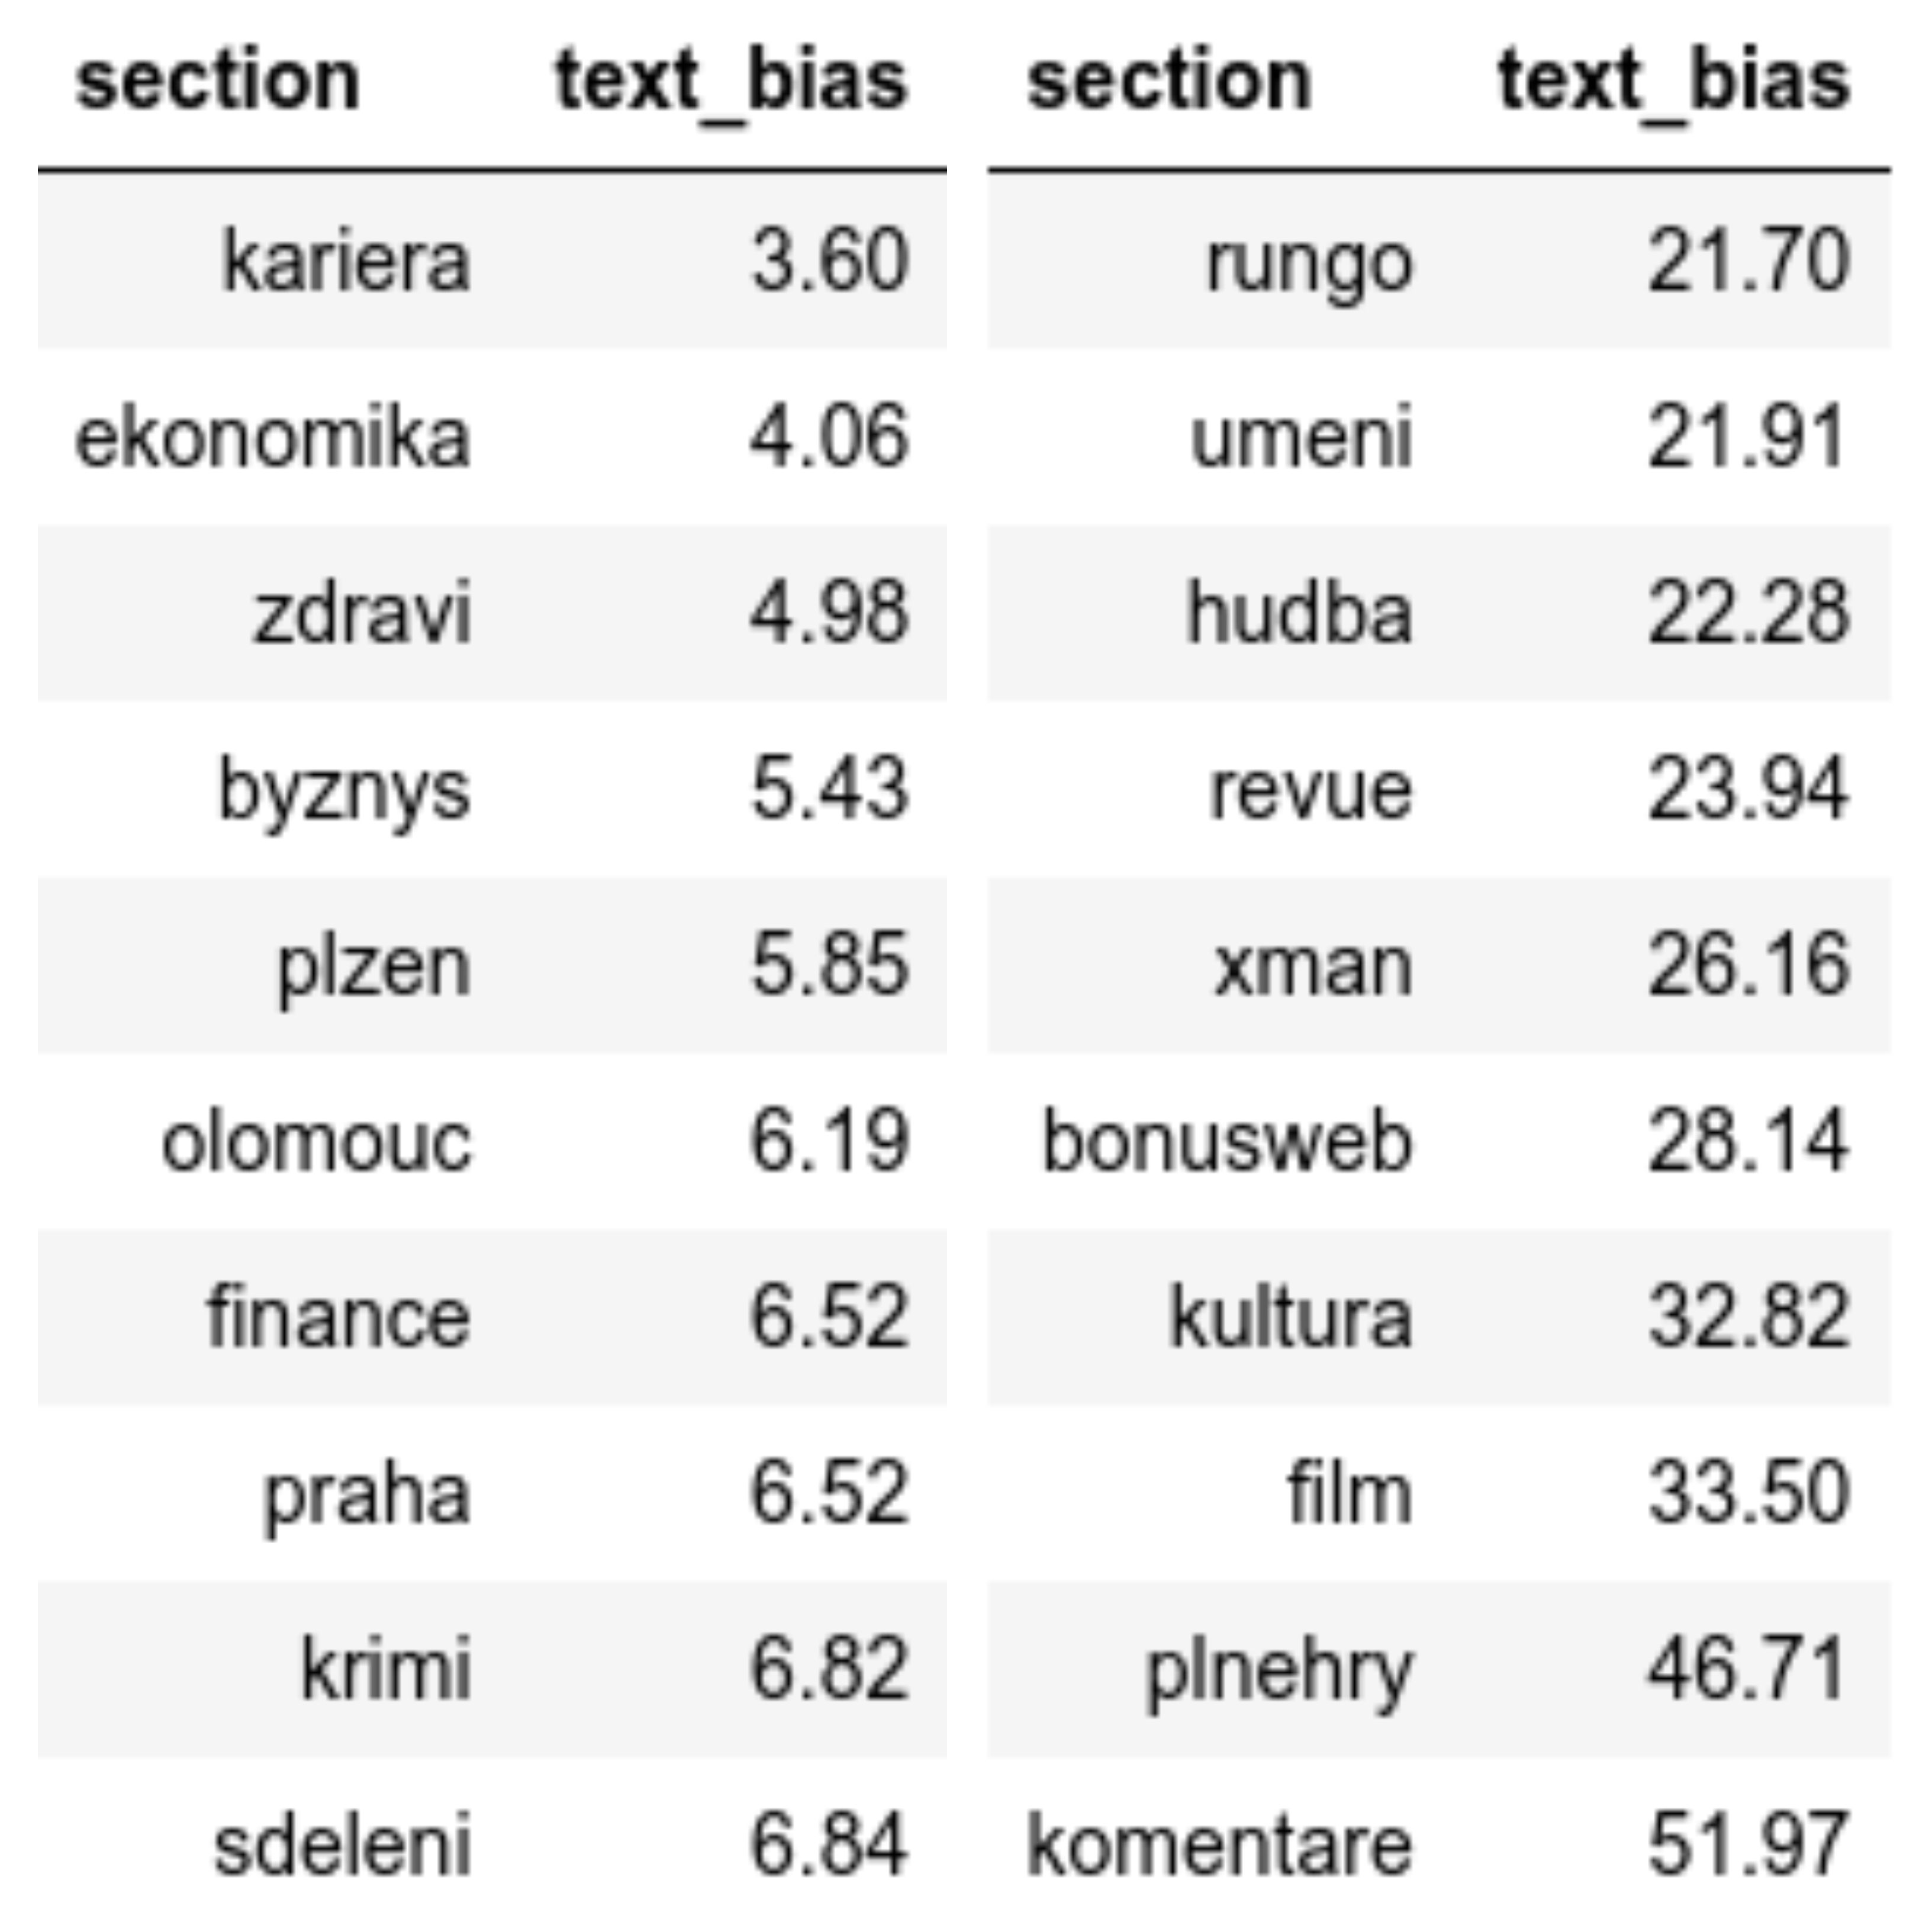
\includegraphics[scale=0.2]{my_modules/multimedia/inference/sections.jpg}
%  \caption{Ten least and ten most biased sections.}
%  \label{fig:sections}
%\end{figure}

\begin{figure}%
    \centering
    \subfloat[\centering in Czech]{{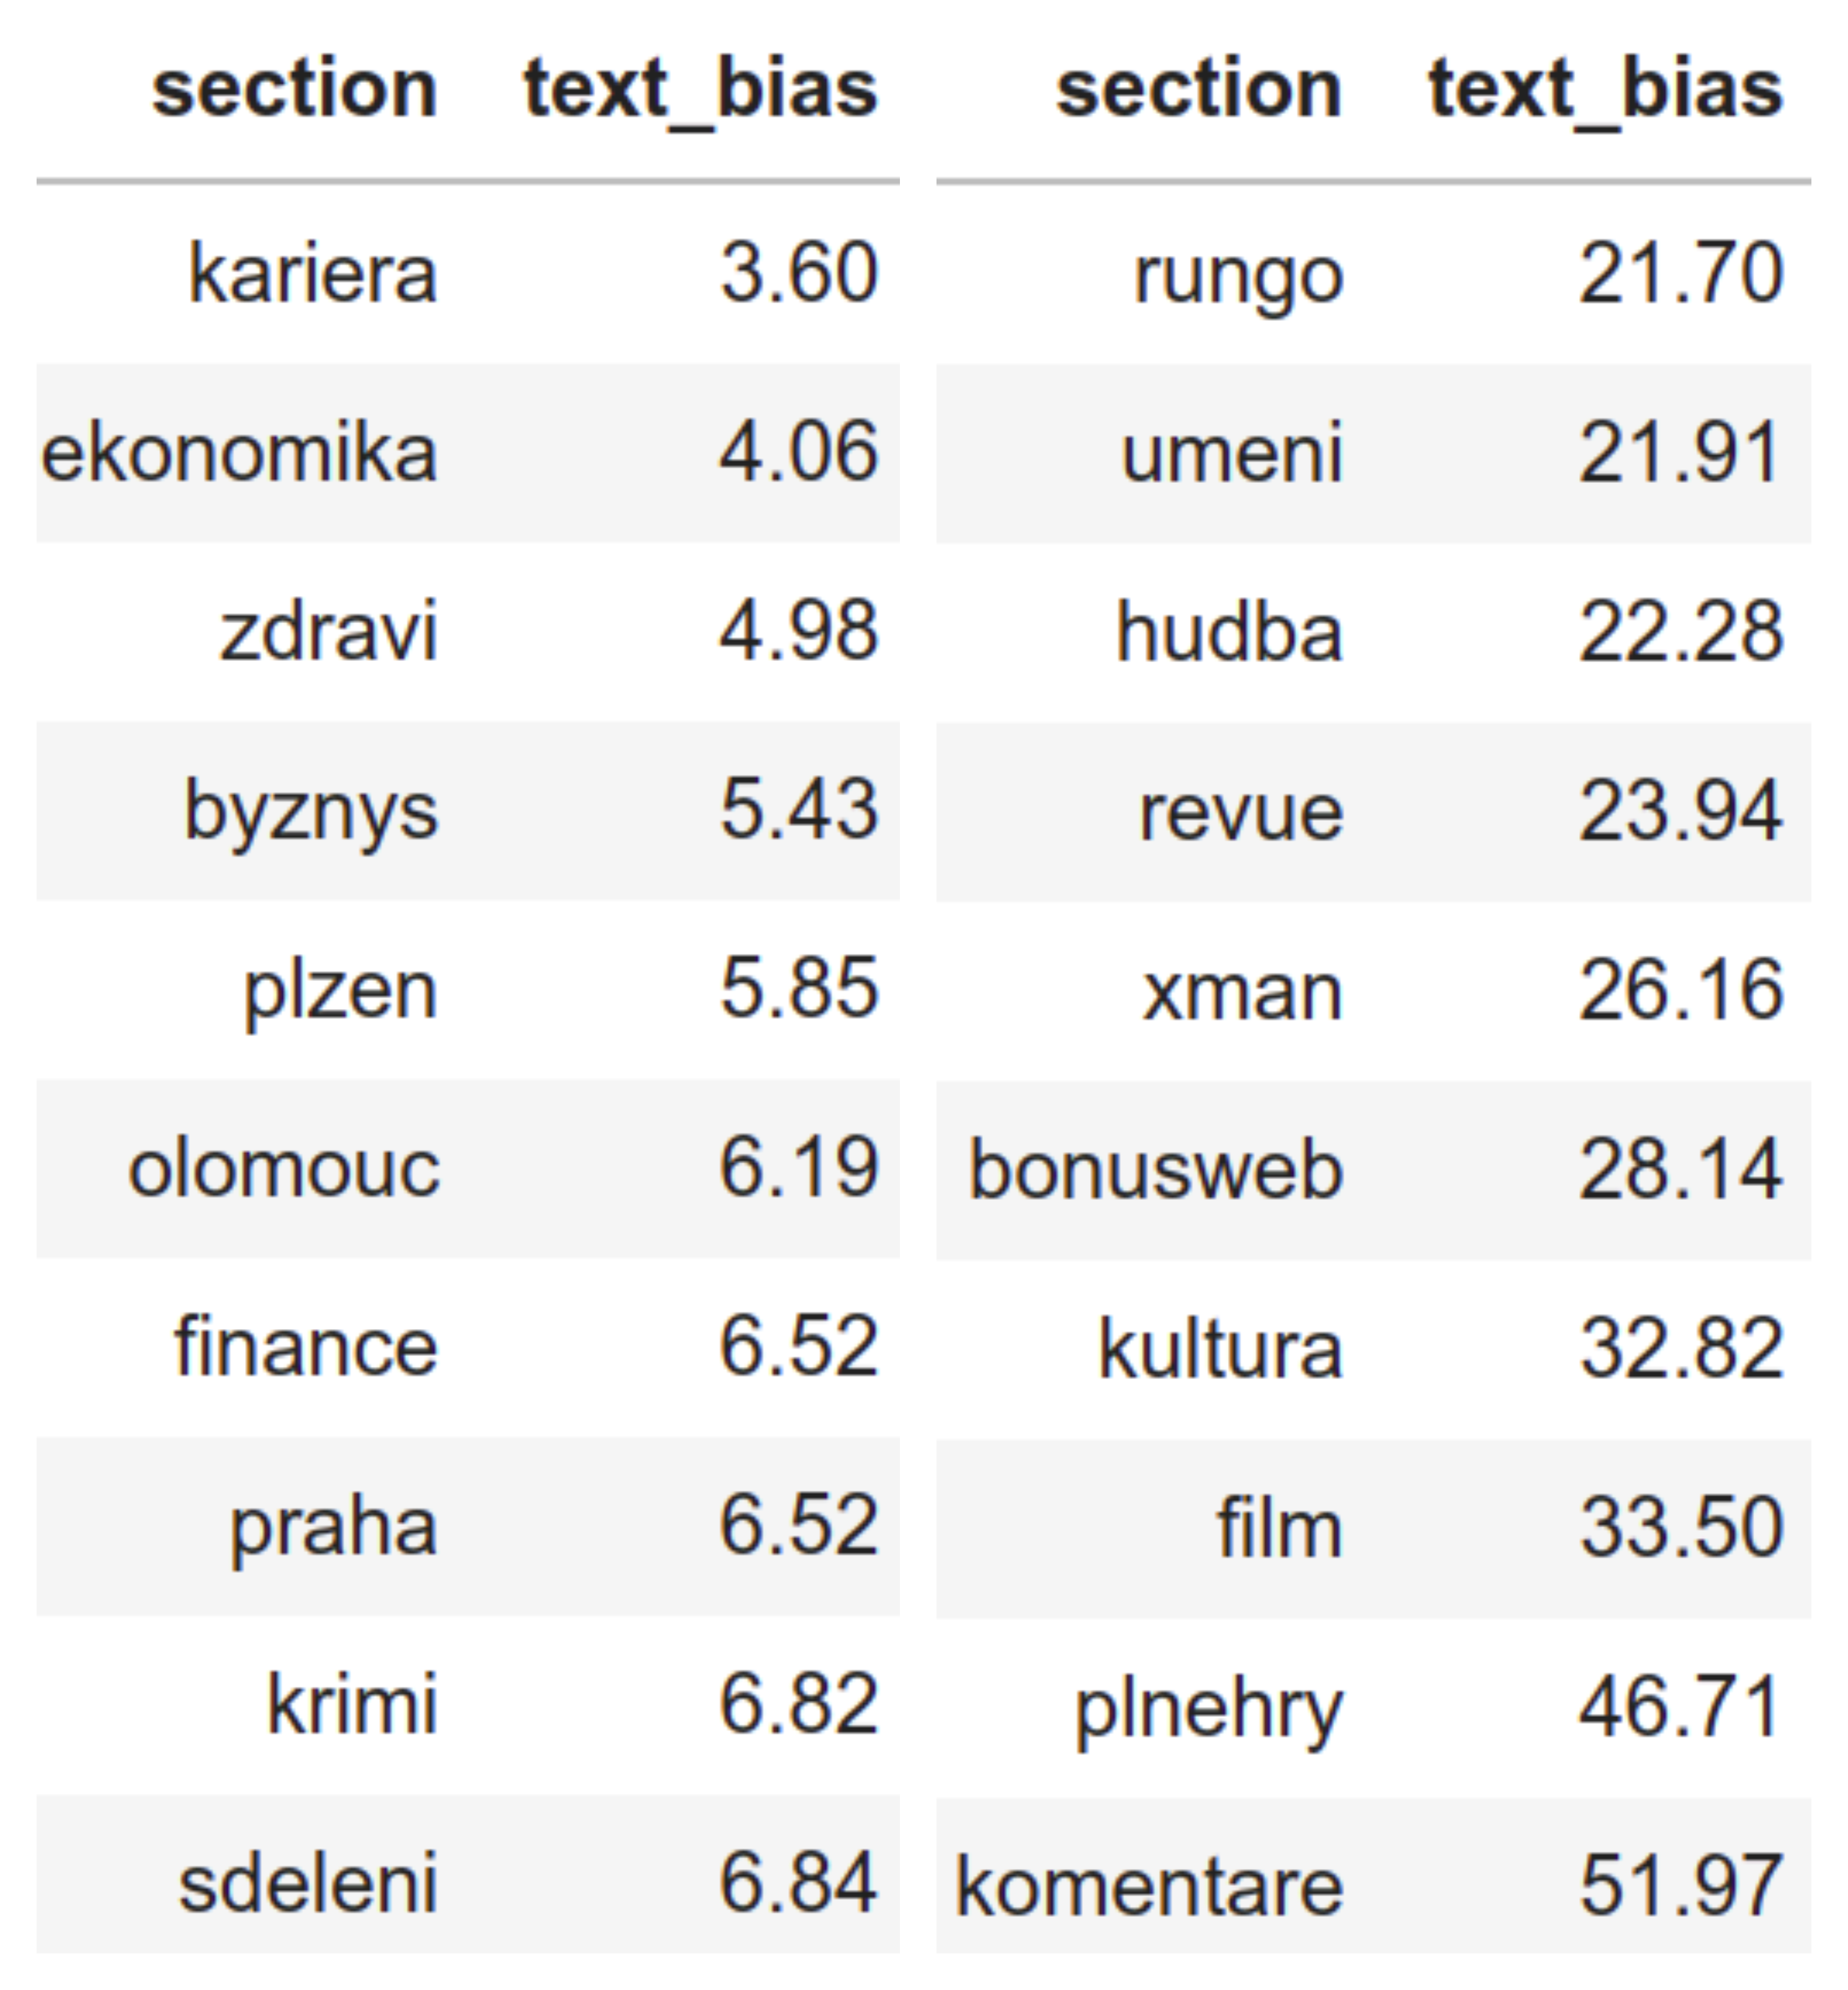
\includegraphics[height=5cm]{my_modules/multimedia/inference/sections_cs.png} }}%
    \qquad
    \subfloat[\centering in English]{{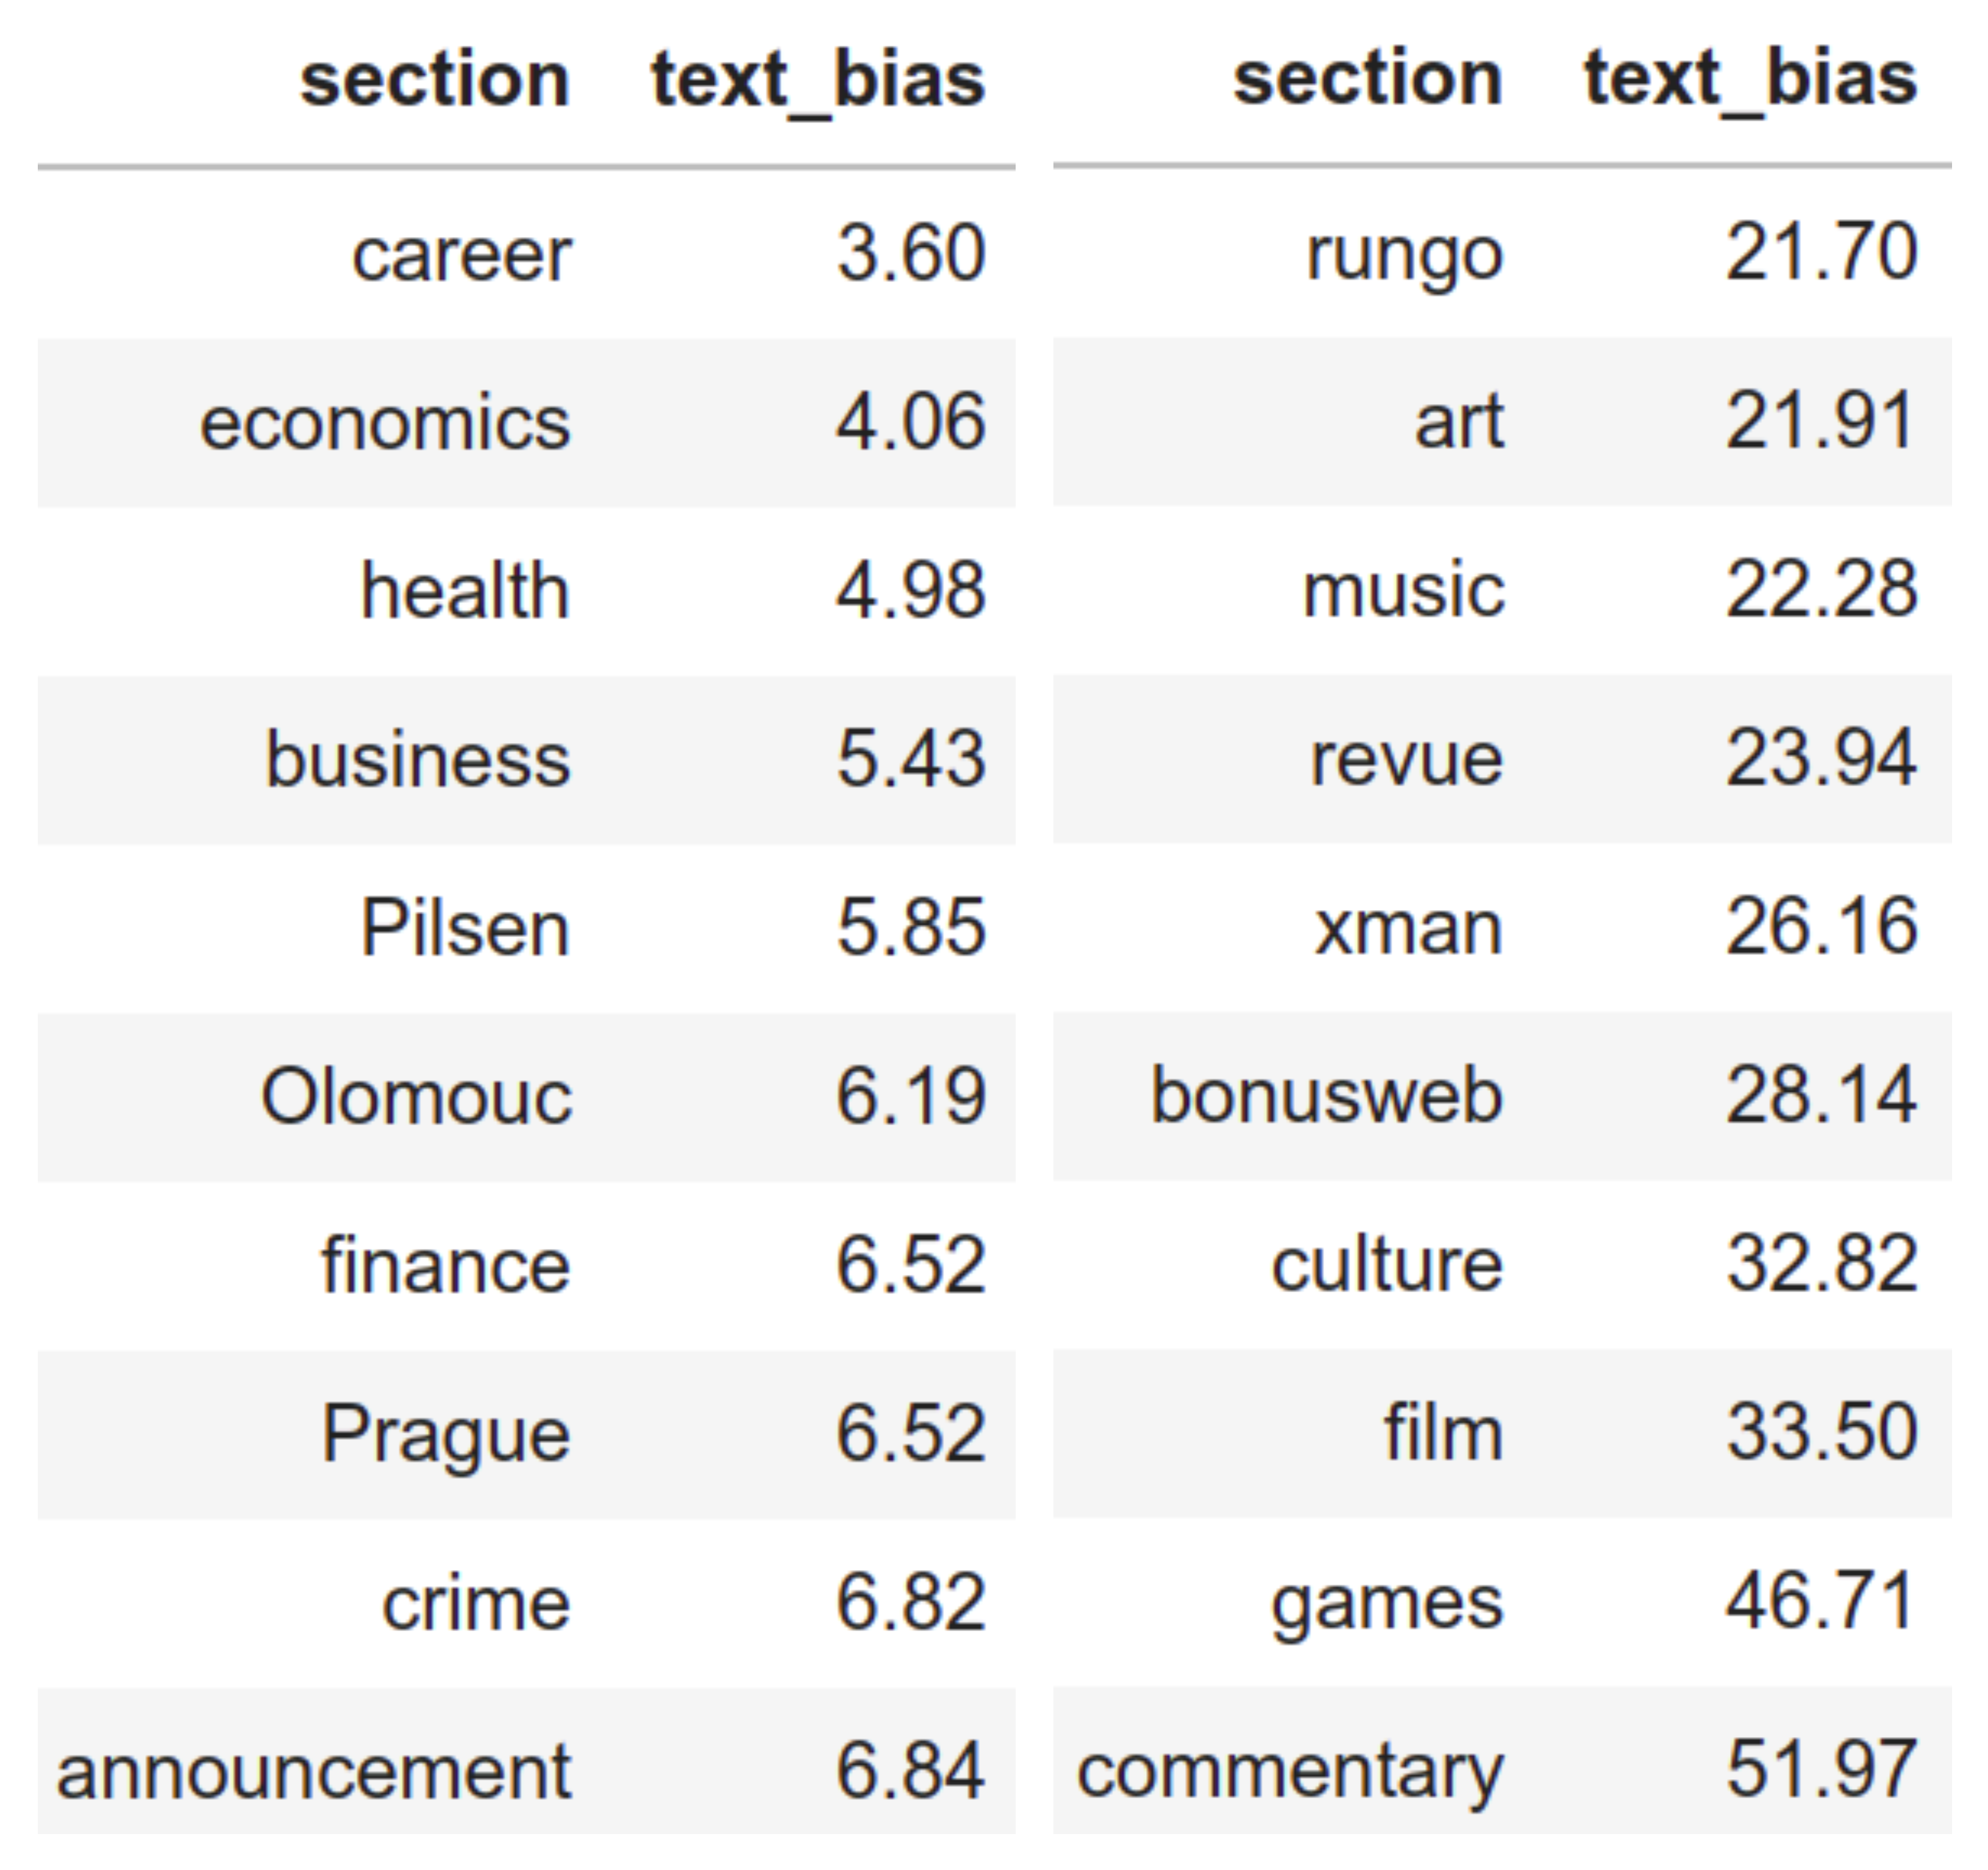
\includegraphics[height=5cm]{my_modules/multimedia/inference/sections_en.png} }}%
    \caption{Ten least and ten most biased sections}%
    \label{fig:sections}%
\end{figure}



%%%%%%%%%%%%%%%%%%%%%%%%%%%%%%%% DENIK %%%%%%%%%%%%%%%%%%%%%%%%%%%%%%%%%%%%%%%%%%%%%%



\subsection{Denik.cz experiments}
Finally, a progression of the media bias over time is examined. Because a distribution of the domains across the years was highly imbalanced, I decided to examine only the denik.cz domain.

To make the results as clear as possible, I only used data from one section. denik.cz data include articles from the years 2007 to 2016. For each year, 350 articles were randomly sampled and the \verb|text_bias| was averaged. A graph of the progression can be seen in figure \ref{fig:denik_years}. I used a linear regression model to fit a line through the data points to highlight the trend.

Additionally, the same statistics, but with respect to months, is shown in figure \ref{fig:months_clean}. A blue stripe represents a confidence interval.

The experiment has shown a decreasing trend in media bias over a period of ten years. The inspection of this result and its possible causes is beyond the scope of this thesis and beyond the scope of the subject of media bias classification. 


\begin{figure}[h]

  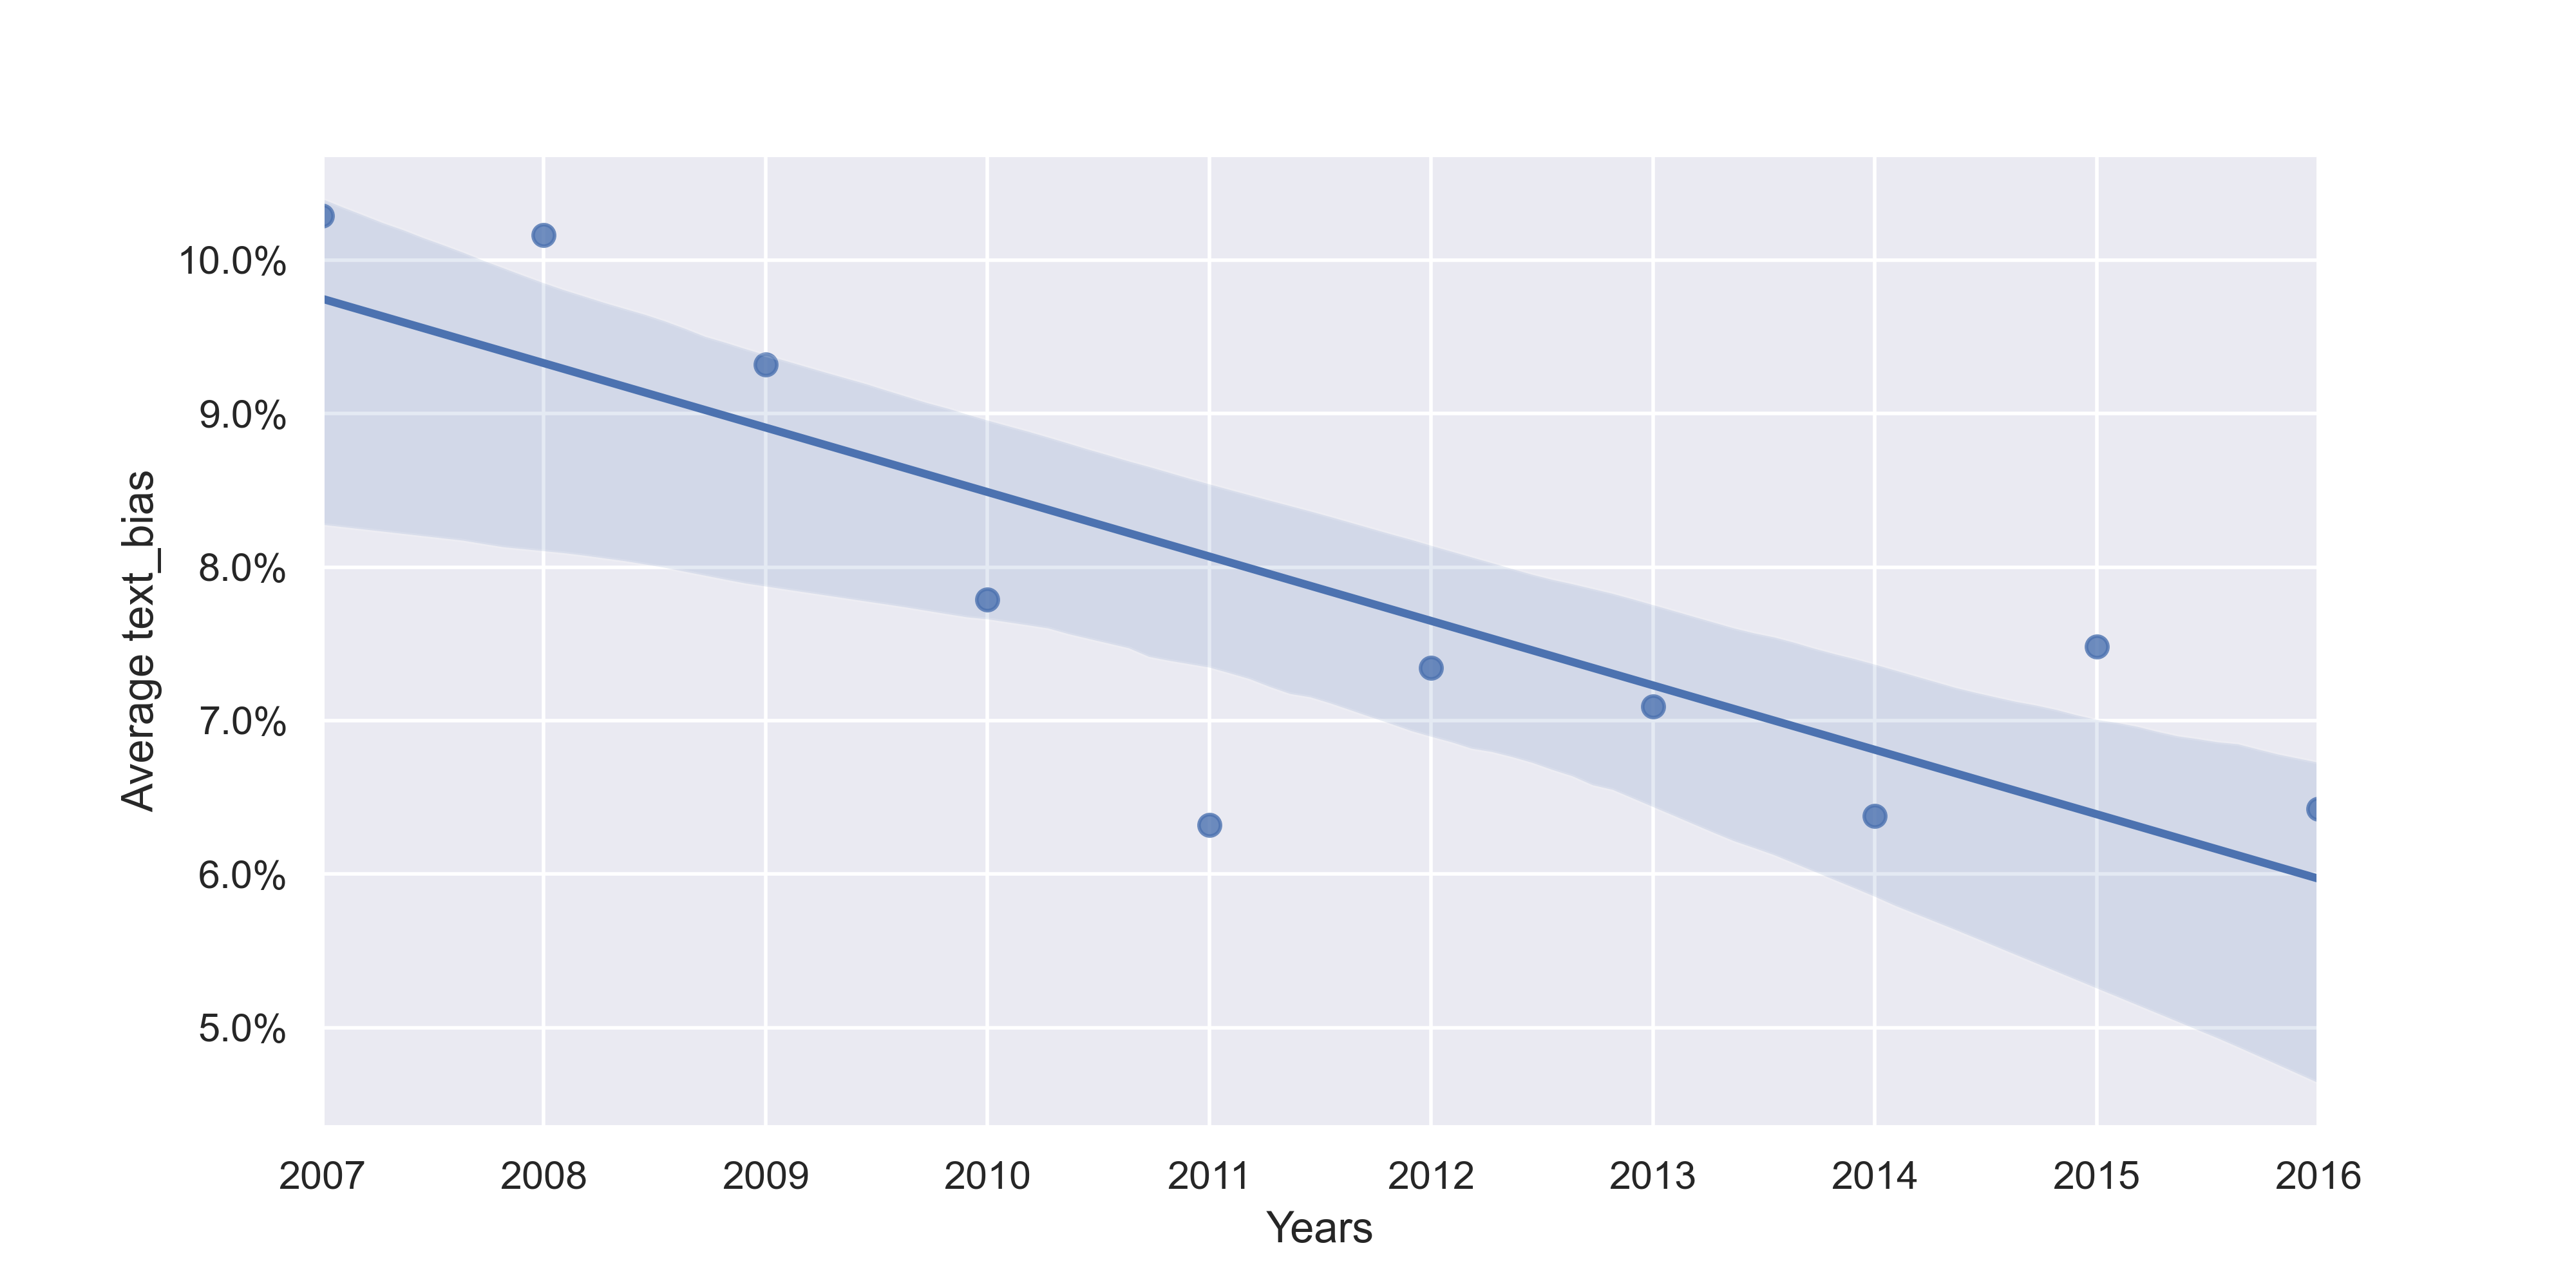
\includegraphics[scale=0.5]{my_modules/multimedia/inference/denik_years.png}
  \caption{Progression of text bias of denik.cz over ten years.}
  \label{fig:denik_years}

\end{figure}


\begin{figure}[h]

  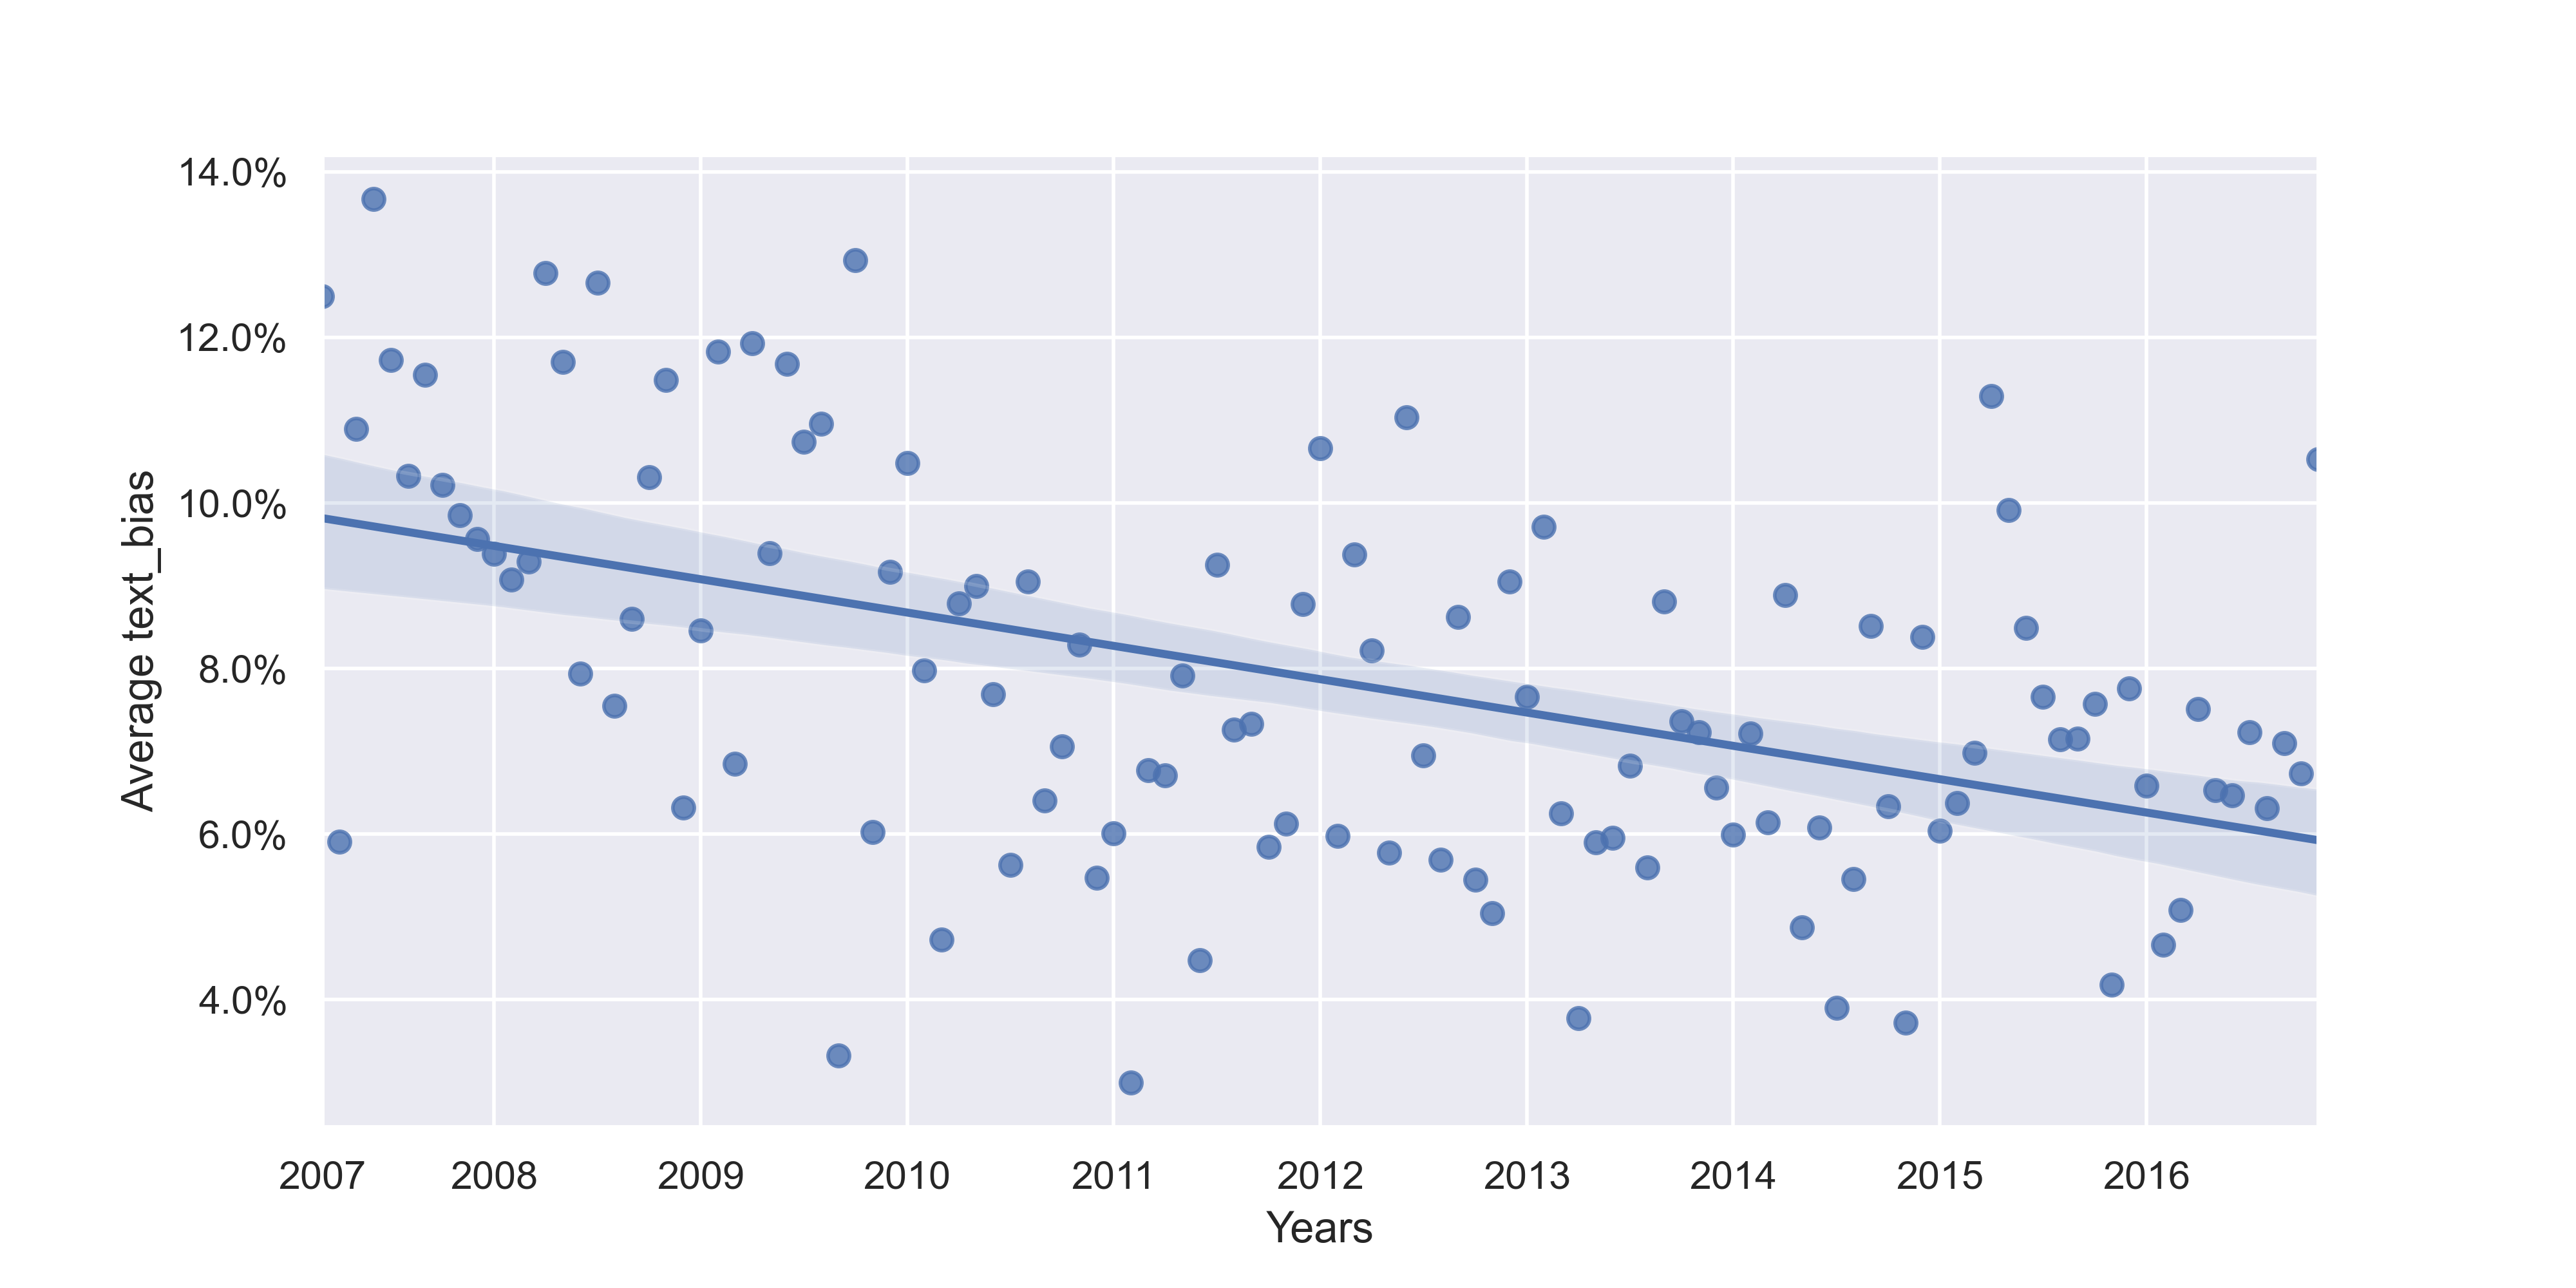
\includegraphics[scale=0.5]{my_modules/multimedia/inference/denik_months2_clean.png}
  \caption{Progression of text bias of denik.cz over ten years. The bias is averaged over months.}
  \label{fig:months_clean}
\end{figure}





\section{Discussion}
Even though these inference experiments have shown some interesting properties of the news, the data has some minor issues in this context. 

For example, not all commentary articles are marked as commentary in the data. Also quoting of reported speech is sometimes missing. 

On top of it, the classifier has around 80\% accuracy (\ref{classifier}), therefore these results should be taken with a grain of salt.

\newpage

%%%%%%%%%%%%%%%%%%%%%%%%%%%%%%%% APP %%%%%%%%%%%%%%%%%%%%%%%%%%%%%%%%%%%%%%%%%%%%%%%%%%%%%%%%%%%%%%%

\section{Application}
Additionally, I provide a simple web demo application for the reader to experiment with\footnote{\url{https://huggingface.co/spaces/horychtom/czech_media_bias_detection}}. The app runs on HuggingFace's spaces\footnote{\url{https://huggingface.co/spaces}} which is a free hosting service for demonstrating \gls{ml} applications. For the frontend, Gradio\footnote{\url{https://gradio.app/}} was used.

The user can insert arbitrary text in Czech language (text in other languages will result in meaningless outcomes). The text is then split into sentences and classified individually.

The application shows the results in two output windows; the first one \textit{classification} displays inserted text with highlighted labels. The second one, \textit{bias ratio}, displays the percentage of biased sentences in the text.

An example can be seen in figure \ref{fig:demodemo}. 
Classification of a news article can be seen in Appendix \ref{classified_article}.

\begin{figure}
\makebox[\textwidth][c]{
  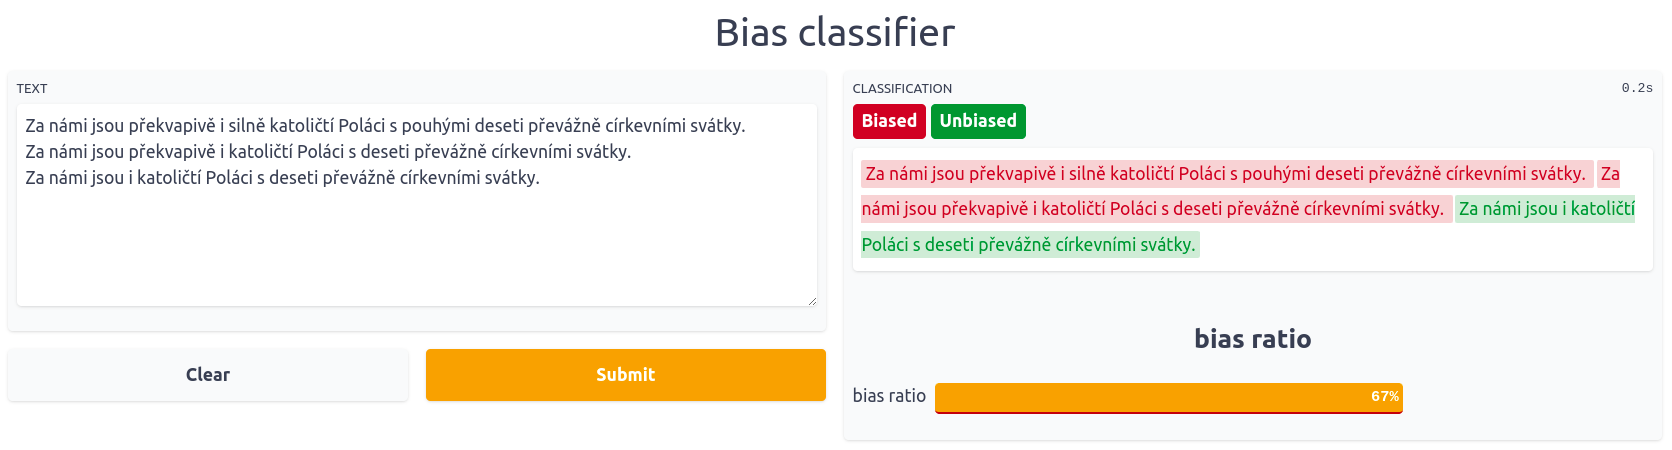
\includegraphics[scale=0.3]{my_modules/multimedia/bias_classif_demo.png}
  \caption{Example of the bias classifier demo usage.}
  \label{fig:demodemo}
  }
\end{figure}



